\chapter{概率分布的弱收敛}
\label{chap:weak-convergence-of-distributions}

第~\ref{chap:common-distributions}章把一块钢板分成$n$格，每格以概率$2/n$出现划痕，划痕数$X_n\sim\operatorname{Bin}(n,2/n)$。格子越分越细，$X_n$的质量表越来越像$\operatorname{Poisson}(2)$的质量表。这里“越来越像”的对象是什么？每个$n$对应一次不同的试验，$X_n$与一个Poisson计数$N$并没有放在同一个样本空间里，差$X_n-N$无从谈起。第~\ref{chap:random-variable-convergence}章的几种收敛都要求共同的样本点，在这里都用不上。能比较的只有分布本身。

再看一个例子。$U_n$在$\{1/n,2/n,\dots,1\}$上等可能取值，每个点的质量都是$1/n$。$n$增大时，每个点的质量趋于零，而$\operatorname{Unif}(0,1)$在每个点的质量本来就是零，逐点比较质量得不出任何信息。可是把$U_n$的直方图画出来，它越来越平，形状逼近$[0,1]$上的均匀密度。可见分布的接近不能简单地定义为质量表逐点接近，需要一种既能处理离散到连续、又只看分布的比较方式。

本章围绕三个问题展开。第一，分布“趋近”应当怎样定义：用有界连续函数的平均作比较，并由此得到事件概率与分布函数的判据。第二，怎样判断一列分布有极限、极限是谁：用紧性防止概率质量逃到无穷远，从而取得收敛子列；再用特征函数识别极限，把独立和化成乘积。矩母函数在附加条件下提供另一种表示。第三，已有的极限怎样传递：经过连续映射、拼成联合分布、代入无界函数的期望时，哪些结论保留，各要什么条件。下一章的中心极限定理将用到这里的全部工具。

\section{弱收敛的定义}
\label{sec:weak-definition}

设$P_1,P_2,\dots$与$P$都是$\mathbb{R}^{d}$上的概率分布，即Borel集族$\mathcal{B}(\mathbb{R}^{d})$上的概率测度。我们要给“$P_n$趋近$P$”一个确切的含义，它只用到这些分布，与产生它们的样本空间无关。先用观测函数的平均作比较，得到定义；再把它与第~\ref{chap:random-variable-convergence}章在共同样本空间上的依概率收敛作对照。

\subsection{分布与测试函数}
\label{sec:weak-test-functions}

比较两个分布，一个直接的办法是选定一个观测函数$f$，看两个分布下$f$的平均
\[
 \int f\,\mathrm{d}P_n\quad\text{与}\quad\int f\,\mathrm{d}P .
\]
把分布看成总量为一的质量，$\int f\,\mathrm{d}P$就是用$f$加权后的总质量。若$f$是某个区间的示性函数，读数就是落在区间里的质量，直方图的每一根柱正是这样一次读数。如果对足够多的$f$读数都接近，就可以说两个分布接近。

问题在于选哪些$f$。第一个要求是有界。对有界的$f$，任何概率分布下的平均都有定义，并且读数的绝对值不超过$\sup\lvert f\rvert$。若允许无界的$f$，例如$f(x)=x$，有的分布（如第~\ref{chap:common-distributions}章的Cauchy分布）根本没有这个平均；第~\ref{sec:weak-integral-limits}节还会看到，极少的质量跑到远处，就能让无界函数的读数变化很大。

第二个要求是连续。设$P_n$是集中在$1/n$的单点分布，$P$集中在$0$。两个质点的位置只差$1/n$，我们希望说$P_n$趋近$P$。若用$f=\mathbf{1}_{(0,\infty)}$读数，$P_n$下的平均恒为$1$，$P$下却是$0$。示性函数在$0$处跳跃，把“稍偏右”与“恰在$0$”截然分开。连续函数对位置的微小变动只给出微小变化：
\[
 \int f\,\mathrm{d}P_n=f(1/n)\longrightarrow f(0)=\int f\,\mathrm{d}P .
\]

把$\mathbb{R}^{d}$上全体有界连续实函数记作$C_b(\mathbb{R}^{d})$。按上面两条要求，用它们作为比较分布的读数。

\begin{definition}[弱收敛与依分布收敛]
\label{def:weak-convergence}
设$P_n$（$n\geq1$）与$P$是$\mathbb{R}^{d}$上的概率分布。若对每个$f\in C_b(\mathbb{R}^{d})$，
\begin{equation}
 \lim_{n\to\infty}\int f\,\mathrm{d}P_n=\int f\,\mathrm{d}P ,
 \label{eq:weak-definition}
\end{equation}
则称$P_n$\term{弱收敛}（weak convergence）到$P$，记作$P_n\xrightarrow{\mathrm{w}}P$。设随机向量$\bm{X}_n$定义在概率空间$(\Omega_n,\mathcal{F}_n,\mathbb{P}_n)$上，$\bm{X}$定义在$(\Omega,\mathcal{F},\mathbb{P})$上。若$P_{\bm{X}_n}\xrightarrow{\mathrm{w}}P_{\bm{X}}$，即对每个$f\in C_b(\mathbb{R}^{d})$都有
\begin{equation}
 \lim_{n\to\infty}\mathbb{E}\bigl[f(\bm{X}_n)\bigr]=\mathbb{E}\bigl[f(\bm{X})\bigr] ,
 \label{eq:weak-convergence-in-distribution}
\end{equation}
则称$\bm{X}_n$\term{依分布收敛}（convergence in distribution）到$\bm{X}$，记作$\bm{X}_n\xrightarrow{\mathrm{d}}\bm{X}$，也写作$\bm{X}_n\xrightarrow{\mathrm{d}}P_{\bm{X}}$。
\end{definition}

式~\eqref{eq:weak-convergence-in-distribution}左边的期望在$\Omega_n$上计算，为简洁不写下标。$f$叫作\term{测试函数}（test function）。这个定义的要点是：$\bm{X}_n$与$\bm{X}$可以定义在不同的样本空间上，比较只通过它们的分布进行。“随机变量依分布收敛”只是“分布弱收敛”的另一种说法，它不断言$\bm{X}_n$的取值与$\bm{X}$的取值越来越近，因为$\bm{X}_n-\bm{X}$可能根本没有定义。

\paragraph{格点上的均匀分布}
回到章首的$U_n$。对$f\in C_b(\mathbb{R})$，
\[
 \mathbb{E}\bigl[f(U_n)\bigr]=\frac1n\sum_{k=1}^{n}f\Bigl(\frac kn\Bigr) .
\]
这正是$f$在$[0,1]$上取右端点的Riemann和。$f$在$[0,1]$上连续，因而可积，Riemann和收敛到积分（可参考\BookChapterRef{chap:univariate-integration}{卷一第7章“一元函数的积分”}）。设$U\sim\operatorname{Unif}(0,1)$，于是
\[
 \lim_{n\to\infty}\mathbb{E}\bigl[f(U_n)\bigr]=\int_0^1f(x)\,\mathrm{d}x=\mathbb{E}\bigl[f(U)\bigr] ,
\]
即$U_n\xrightarrow{\mathrm{d}}\operatorname{Unif}(0,1)$。

取一个具体的测试函数$f(x)=\min(x^2,1)$，它在$[0,1]$上就是$x^2$。由平方和公式，
\[
 \mathbb{E}\bigl[f(U_n)\bigr]=\frac{1}{n^{3}}\sum_{k=1}^{n}k^{2}=\frac{(n+1)(2n+1)}{6n^{2}} .
\]
$n=5,10,50$时依次为
\[
 0.4400,\qquad 0.3850,\qquad 0.3434,
\]
逐渐接近$\int_0^1x^2\,\mathrm{d}x=1/3$。图~\ref{fig:weak-lattice-uniform}(a)中，柱的面积之和就是这个读数；(b)画出读数随$n$的变化。每个格点的质量$1/n$趋于零，读数却收敛：弱收敛比较的是质量的整体摆放，而不是单点的质量。

\begin{BookInlineFigure}
 \centering
 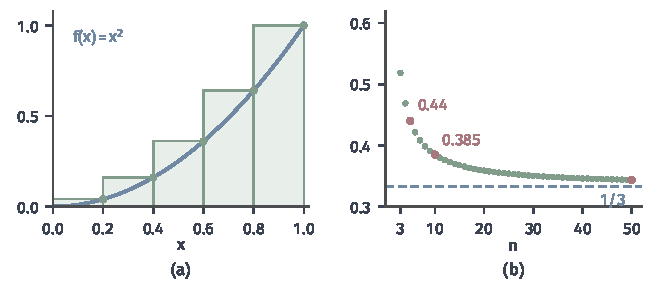
\includegraphics[width=112mm]{figures/07-probability/03-probability-limits/matplotlib/weak-lattice-uniform/figure.pdf}
 \caption{格点均匀分布的弱收敛。(a)$n=5$，浅绿柱宽$1/5$、高$f(k/5)$（绿点），面积之和为$\mathbb{E}[f(U_5)]=0.44$；蓝线为测试函数$f(x)=x^2$，其下面积为$1/3$。(b)$\mathbb{E}[f(U_n)]$随$n$的变化（绿点），蓝色虚线为极限$1/3$。}
 \label{fig:weak-lattice-uniform}
\end{BookInlineFigure}

\paragraph{极限的唯一性}
一列数的极限唯一。对分布也应如此，否则“极限分布”就不是一个确定的对象。这归结为：有界连续函数的读数能否区分两个分布。下面构造一族连续函数，从上方逼近闭集的示性函数。

对闭集$F\subset\mathbb{R}^{d}$，记点$\bm{x}$到$F$的距离为
\[
 \operatorname{dist}(\bm{x},F)=\inf_{\bm{y}\in F}\lVert\bm{x}-\bm{y}\rVert_2 ,
\]
并令
\begin{equation}
 f_k(\bm{x})=\max\bigl(0,\,1-k\operatorname{dist}(\bm{x},F)\bigr),\qquad k=1,2,\dots .
 \label{eq:weak-closed-approx}
\end{equation}
由三角不等式，距离函数满足
\[
 \lvert\operatorname{dist}(\bm{x},F)-\operatorname{dist}(\bm{y},F)\rvert\leq\lVert\bm{x}-\bm{y}\rVert_2 ,
\]
所以$f_k$连续，并且是Lipschitz常数为$k$的Lipschitz函数。它在$F$上等于$1$，在距$F$不小于$1/k$处等于$0$，取值在$[0,1]$中。

\begin{lemma}[有界连续函数确定分布]
\label{lem:weak-uniqueness}
设$P,Q$是$\mathbb{R}^{d}$上的概率分布。若对每个$f\in C_b(\mathbb{R}^{d})$都有$\int f\,\mathrm{d}P=\int f\,\mathrm{d}Q$，则$P=Q$。因此弱收敛的极限唯一：若$P_n\xrightarrow{\mathrm{w}}P$且$P_n\xrightarrow{\mathrm{w}}Q$，则$P=Q$。
\end{lemma}

\begin{proof}
取闭集$F$与式~\eqref{eq:weak-closed-approx}中的$f_k$。若$\bm{x}\in F$，则$f_k(\bm{x})=1$。若$\bm{x}\notin F$，因$F$闭，$\operatorname{dist}(\bm{x},F)>0$，当$k>1/\operatorname{dist}(\bm{x},F)$时$f_k(\bm{x})=0$。所以$f_k$逐点不增地趋于$\mathbf{1}_F$。

$0\leq f_k\leq1$，由支配收敛定理，
\[
 P(F)=\lim_{k\to\infty}\int f_k\,\mathrm{d}P=\lim_{k\to\infty}\int f_k\,\mathrm{d}Q=Q(F) .
\]
于是$P$与$Q$在全体闭集上相等。闭集族对有限交封闭，并且生成$\mathcal{B}(\mathbb{R}^{d})$。由第~\ref{chap:probability-spaces}章测度的唯一性定理，$P=Q$。

若$P_n$同时弱收敛到$P$和$Q$，则对每个$f\in C_b(\mathbb{R}^{d})$，$\int f\,\mathrm{d}P$与$\int f\,\mathrm{d}Q$是同一数列的极限，二者相等，再由前半部分得$P=Q$。
\end{proof}

\paragraph{同分布而样本不接近}
依分布收敛不涉及样本，下面的例子把这一点推到极端。取$\Omega=[0,1]$，$\mathbb{P}$为长度，令
\[
 X(\omega)=\omega,\qquad Y(\omega)=1-\omega .
\]
对$0\leq x\leq1$，$\mathbb{P}(Y\leq x)=\mathbb{P}(\omega\geq1-x)=x$，所以$X$与$Y$都服从$\operatorname{Unif}(0,1)$。令$X_n=Y$对一切$n$成立，则$X_n$与$X$的分布完全相同，$X_n\xrightarrow{\mathrm{d}}X$平凡地成立。

可是在样本点$\omega$上，$X_n$与$X$相差$\lvert1-2\omega\rvert$，与$n$无关，并且
\[
 \mathbb{P}\bigl(\lvert X_n-X\rvert>1/2\bigr)=\mathbb{P}\bigl(\omega<1/4\text{ 或 }\omega>3/4\bigr)=\frac12 .
\]
图~\ref{fig:weak-same-law}(a)画出这两个$\Omega$上的函数，它们在大部分样本点上相距很远；(b)是它们的直方图，完全一样。这好比两个班的身高分布相同，并不意味着按学号配对的两人身高接近。依分布收敛只比较“分布”这一侧，不管它由哪个函数实现。

\begin{BookInlineFigure}
 \centering
 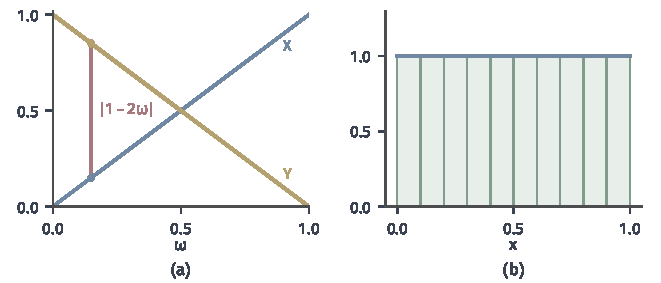
\includegraphics[width=112mm]{figures/07-probability/03-probability-limits/matplotlib/weak-same-law/figure.pdf}
 \caption{同分布而样本不接近。(a)$\Omega=[0,1]$上的$X(\omega)=\omega$（蓝）与$Y(\omega)=1-\omega$（黄），红色竖线段标出一个样本点上的差$\lvert1-2\omega\rvert$。(b)二者各用$\omega$的$2000$个等距点算出的直方图（浅绿），与$\operatorname{Unif}(0,1)$的密度（蓝）一致。}
 \label{fig:weak-same-law}
\end{BookInlineFigure}

\subsection{与依概率收敛的关系}
\label{sec:weak-probability-convergence}

当$\bm{X}_n$与$\bm{X}$定义在同一概率空间上时，第~\ref{chap:random-variable-convergence}章的依概率收敛$\bm{X}_n\xrightarrow{\mathbb{P}}\bm{X}$也有意义：对每个$\varepsilon>0$，事件$\lVert\bm{X}_n-\bm{X}\rVert_2\geq\varepsilon$的概率趋于零。上一个例子说明依分布收敛不能推出依概率收敛。反方向则成立：样本接近时，分布也接近。

\begin{theorem}[依概率收敛蕴含依分布收敛]
\label{thm:weak-prob-implies-dist}
设$\bm{X}_n$与$\bm{X}$是同一概率空间上取值于$\mathbb{R}^{d}$的随机向量。若$\bm{X}_n\xrightarrow{\mathbb{P}}\bm{X}$，则$\bm{X}_n\xrightarrow{\mathrm{d}}\bm{X}$。
\end{theorem}

\begin{proof}
取$f\in C_b(\mathbb{R}^{d})$，记$M=\sup\lvert f\rvert$，任取$\varepsilon>0$。困难在于$f$在整个空间上未必一致连续，所以先把$\bm{X}$限制在一个有界范围内。事件$\{\lVert\bm{X}\rVert_2>r\}$随$r$增大而下降到空集，由概率的连续性，存在$r$使$\mathbb{P}(\lVert\bm{X}\rVert_2>r)<\varepsilon$。

闭球$B=\{\lVert\bm{x}\rVert_2\leq r+1\}$是紧集，$f$在$B$上一致连续。于是存在$\delta\in(0,1)$，使得$\bm{x},\bm{y}\in B$且$\lVert\bm{x}-\bm{y}\rVert_2<\delta$时$\lvert f(\bm{x})-f(\bm{y})\rvert<\varepsilon$。

若$\lVert\bm{X}\rVert_2\leq r$且$\lVert\bm{X}_n-\bm{X}\rVert_2<\delta$，则$\bm{X}$与$\bm{X}_n$都在$B$中，$\lvert f(\bm{X}_n)-f(\bm{X})\rvert<\varepsilon$。其余情形用$\lvert f(\bm{X}_n)-f(\bm{X})\rvert\leq2M$。两部分合起来，
\[
 \bigl\lvert\mathbb{E}[f(\bm{X}_n)]-\mathbb{E}[f(\bm{X})]\bigr\rvert
 \leq\varepsilon+2M\,\mathbb{P}\bigl(\lVert\bm{X}\rVert_2>r\bigr)+2M\,\mathbb{P}\bigl(\lVert\bm{X}_n-\bm{X}\rVert_2\geq\delta\bigr) .
\]
令$n\to\infty$，最后一项趋于零，所以
\[
 \limsup_{n\to\infty}\bigl\lvert\mathbb{E}[f(\bm{X}_n)]-\mathbb{E}[f(\bm{X})]\bigr\rvert\leq\varepsilon+2M\varepsilon .
\]
$\varepsilon$任意，左边为零。
\end{proof}

反方向不成立，离散的例子更直接。设$X\sim\operatorname{Bern}(1/2)$，令$X_n=1-X$。$X_n$也服从$\operatorname{Bern}(1/2)$，所以$X_n\xrightarrow{\mathrm{d}}X$；但$\lvert X_n-X\rvert=1$恒成立，$\mathbb{P}(\lvert X_n-X\rvert\geq1/2)=1$。

\paragraph{极限为常量}
有一种情形反向结论成立：极限分布集中在一个点$\bm{c}$上。常量在任何概率空间上都可以定义，$\bm{X}_n\xrightarrow{\mathbb{P}}\bm{c}$只要求事件$\lVert\bm{X}_n-\bm{c}\rVert_2\geq\varepsilon$的概率趋于零，其中的概率在$\bm{X}_n$所在的空间上计算，所以即使各$\bm{X}_n$在不同的空间上，这个说法也有意义。

\begin{theorem}[依分布趋于常量]
\label{thm:weak-constant-limit}
设$\bm{c}\in\mathbb{R}^{d}$。若$\bm{X}_n\xrightarrow{\mathrm{d}}\bm{c}$，则对每个$\varepsilon>0$，
\begin{equation}
 \lim_{n\to\infty}\mathbb{P}\bigl(\lVert\bm{X}_n-\bm{c}\rVert_2\geq\varepsilon\bigr)=0 ,
 \label{eq:weak-constant-limit}
\end{equation}
即$\bm{X}_n\xrightarrow{\mathbb{P}}\bm{c}$。
\end{theorem}

\begin{proof}
令
\[
 h(\bm{x})=\min\bigl(1,\lVert\bm{x}-\bm{c}\rVert_2/\varepsilon\bigr) .
\]
它有界连续，$h(\bm{c})=0$，并且在$\lVert\bm{x}-\bm{c}\rVert_2\geq\varepsilon$处等于$1$，所以$h$处处不小于偏离事件$\{\lVert\bm{x}-\bm{c}\rVert_2\geq\varepsilon\}$的示性函数。取期望，
\[
 \mathbb{P}\bigl(\lVert\bm{X}_n-\bm{c}\rVert_2\geq\varepsilon\bigr)\leq\mathbb{E}\bigl[h(\bm{X}_n)\bigr]\longrightarrow h(\bm{c})=0 .
\]
\end{proof}

证明用一个连续函数从上方压住“偏离$\bm{c}$至少$\varepsilon$”的示性函数，见图~\ref{fig:weak-constant-limit}。常量之所以特殊，是因为它没有随机性需要与$\bm{X}_n$配对：知道$\bm{X}_n$的分布集中到$\bm{c}$附近，就知道$\bm{X}_n$本身以大概率在$\bm{c}$附近。第~\ref{sec:weak-slutsky}节的Slutsky定理要用到这一点。

\begin{BookInlineFigure}
 \centering
 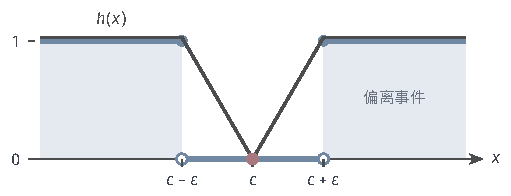
\includegraphics[width=86.6mm]{figures/07-probability/03-probability-limits/tikz/weak-constant-limit/figure.pdf}
 \caption{常量极限的证明。深灰折线为$h(x)=\min(1,\lvert x-c\rvert/\varepsilon)$，它连续且在$c$处为零；浅蓝区域为偏离事件$\{\lvert x-c\rvert\geq\varepsilon\}$，其示性函数（蓝色粗线）处处不超过$h$。}
 \label{fig:weak-constant-limit}
\end{BookInlineFigure}


\section{事件概率判据}
\label{sec:weak-event-criteria}

实际关心的往往是事件的概率：$X_n\leq x$的概率是否趋于$X\leq x$的概率，$\bm{X}_n$落在某个区域的概率是否收敛。事件的示性函数有界，却不连续，定义~\ref{def:weak-convergence}不能直接用于它。

两个例子说明困难确实存在。单点分布$\delta_{1/n}$趋于$\delta_0$，取$A=(0,\infty)$，则$\delta_{1/n}(A)=1$而$\delta_0(A)=0$；取$A=(-\infty,0]$，结果反过来。格点均匀分布$U_n\xrightarrow{\mathrm{d}}U\sim\operatorname{Unif}(0,1)$，取$A$为$[0,1]$中有理数的全体，则$\mathbb{P}(U_n\in A)=1$对一切$n$成立，而$\mathbb{P}(U\in A)=0$。

两个反例有共同的原因。记$\partial A$为$A$的边界，即闭包去掉内部。第一个例子中$\partial A=\{0\}$，极限分布在这里有质量$1$。第二个例子中，有理数的闭包是$[0,1]$，内部是空集，边界是整个$[0,1]$，极限分布在边界上的质量也是$1$。质量可以在极限过程中移到边界上，从$A$的一侧挪到另一侧，见图~\ref{fig:weak-boundary-mass}。本节证明：只有这种情形会出问题。

\begin{BookInlineFigure}
 \centering
 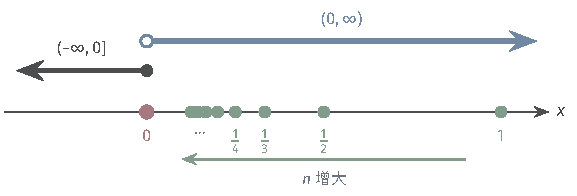
\includegraphics[width=97.6mm]{figures/07-probability/03-probability-limits/tikz/weak-boundary-mass/figure.pdf}
 \caption{质量移到边界上。绿点为$\delta_{1/n}$的质点位置$1,\,1/2,\,1/3,\dots$，红点为极限$\delta_0$的质点。蓝色为开集$(0,\infty)$，深灰为闭集$(-\infty,0]$，二者的公共边界是$0$：每个$\delta_{1/n}$都把全部质量放在开集里，极限却把它放在闭集里。}
 \label{fig:weak-boundary-mass}
\end{BookInlineFigure}

\subsection{Portmanteau定理}
\label{sec:weak-portmanteau}

图~\ref{fig:weak-boundary-mass}还显示了一个方向性：质量从开集一侧移到边界，闭集$(-\infty,0]$在极限中多得了质量，开集$(0,\infty)$在极限中失去了质量。一般地，极限过程中闭集的概率只能“突然增加”，开集的概率只能“突然减少”。用连续函数逼近示性函数，可以把这个直观变成不等式。

闭集$F$的示性函数由式~\eqref{eq:weak-closed-approx}的$f_k$从上方逼近。对开集$G$，补集$G^{\mathrm{c}}$闭，令
\begin{equation}
 g_k(\bm{x})=\min\bigl(1,\,k\operatorname{dist}(\bm{x},G^{\mathrm{c}})\bigr),\qquad k=1,2,\dots .
 \label{eq:weak-open-approx}
\end{equation}
$g_k$连续，取值在$[0,1]$中，在$G^{\mathrm{c}}$上为零，并且逐点不减地趋于$\mathbf{1}_G$：$\bm{x}\in G$时$\operatorname{dist}(\bm{x},G^{\mathrm{c}})>0$，$k$足够大后$g_k(\bm{x})=1$。图~\ref{fig:weak-portmanteau-approx}画出了区间上的这两族函数。

\begin{BookInlineFigure}
 \centering
 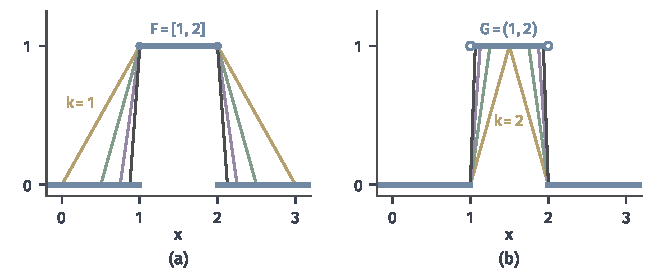
\includegraphics[width=112mm]{figures/07-probability/03-probability-limits/matplotlib/weak-portmanteau-approx/figure.pdf}
 \caption{用连续函数逼近示性函数。(a)闭区间$F=[1,2]$，$f_k$从上方逼近$\mathbf{1}_F$（蓝色粗线），黄、绿、紫、深灰依次为$k=1,2,4,8$。(b)开区间$G=(1,2)$，$g_k$从下方逼近$\mathbf{1}_G$，四种颜色依次为$k=2,4,8,16$。}
 \label{fig:weak-portmanteau-approx}
\end{BookInlineFigure}

\begin{theorem}[Portmanteau定理]
\label{thm:weak-portmanteau}
设$P_n$（$n\geq1$）与$P$是$\mathbb{R}^{d}$上的概率分布。以下五条等价：
\begin{enumerate}
 \item $P_n\xrightarrow{\mathrm{w}}P$；
 \item 对每个有界且Lipschitz连续的$f$，$\int f\,\mathrm{d}P_n\to\int f\,\mathrm{d}P$；
 \item 对每个闭集$F$，$\limsup_{n}P_n(F)\leq P(F)$；
 \item 对每个开集$G$，$\liminf_{n}P_n(G)\geq P(G)$；
 \item 对每个满足$P(\partial A)=0$的Borel集$A$，$P_n(A)\to P(A)$。
\end{enumerate}
\end{theorem}

\begin{proof}
(1)$\Rightarrow$(2)：有界Lipschitz函数是有界连续函数。

(2)$\Rightarrow$(3)：式~\eqref{eq:weak-closed-approx}的$f_k$有界且Lipschitz，并且$f_k\geq\mathbf{1}_F$。固定$k$，
\[
 \limsup_{n\to\infty}P_n(F)\leq\lim_{n\to\infty}\int f_k\,\mathrm{d}P_n=\int f_k\,\mathrm{d}P .
\]
引理~\ref{lem:weak-uniqueness}的证明已经说明$\int f_k\,\mathrm{d}P\to P(F)$。令$k\to\infty$即得(3)。

(3)$\Leftrightarrow$(4)：$G$为开集当且仅当$G^{\mathrm{c}}$为闭集，并且$P_n(G)=1-P_n(G^{\mathrm{c}})$，所以
\[
 \liminf_{n\to\infty}P_n(G)=1-\limsup_{n\to\infty}P_n(G^{\mathrm{c}})\geq1-P(G^{\mathrm{c}})=P(G) .
\]
反方向同理。

(3)与(4)$\Rightarrow$(5)：记$A^{\circ}$为$A$的内部，$\bar{A}$为闭包，则$A^{\circ}\subset A\subset\bar{A}$，且$\bar{A}\setminus A^{\circ}=\partial A$。由$P(\partial A)=0$得$P(A^{\circ})=P(A)=P(\bar{A})$。于是
\[
 \begin{aligned}
 \limsup_{n\to\infty}P_n(A)&\leq\limsup_{n\to\infty}P_n(\bar{A})\leq P(\bar{A})=P(A),\\
 \liminf_{n\to\infty}P_n(A)&\geq\liminf_{n\to\infty}P_n(A^{\circ})\geq P(A^{\circ})=P(A) .
 \end{aligned}
\]
上极限不超过下极限，所以$P_n(A)\to P(A)$。

(5)$\Rightarrow$(1)：取$f\in C_b(\mathbb{R}^{d})$。式~\eqref{eq:weak-definition}两边对$f$都是线性的，常数函数的读数恒为$1$，所以可以对$f$作正的伸缩与平移，不妨设$0<f<1$。由第~\ref{chap:tail-probabilities}章的尾积分公式，
\[
 \int f\,\mathrm{d}P=\int_0^1P(f>t)\,\mathrm{d}t ,
\]
对$P_n$同样成立。

集合$G_t=\{f>t\}$是开集，闭包含于$\{f\geq t\}$，所以$\partial G_t\subset\{f=t\}$。不同$t$对应的集合$\{f=t\}$互不相交，对每个正整数$m$，满足$P(f=t)\geq1/m$的$t$至多$m$个，所以$P(f=t)>0$的$t$至多可数。除去这些$t$，由(5)得$P_n(G_t)\to P(G_t)$。被积函数取值在$[0,1]$中，可数集长度为零，由支配收敛定理，
\[
 \int_0^1P_n(f>t)\,\mathrm{d}t\longrightarrow\int_0^1P(f>t)\,\mathrm{d}t ,
\]
即$\int f\,\mathrm{d}P_n\to\int f\,\mathrm{d}P$。
\end{proof}

\term{Portmanteau定理}（portmanteau theorem）的名字意为“手提箱”，指把几种等价说法装在一起。五条各有用途。(2)把测试函数缩小到有界Lipschitz函数，第~\ref{sec:weak-slutsky}节要用它。(3)和(4)说明极限中闭集可能多得质量、开集可能失去质量，图~\ref{fig:weak-boundary-mass}中两个不等号都是严格的：$\limsup\delta_{1/n}\bigl((-\infty,0]\bigr)=0<1$，$\liminf\delta_{1/n}\bigl((0,\infty)\bigr)=1>0$。(5)给出事件概率真正收敛的条件。

注意(5)中的条件只针对极限分布$P$，不针对$P_n$。格点均匀分布中，$A=[0,1/2]$的边界是$\{0,1/2\}$，$U_n$在$1/2$可能有质量（$n$为偶数时），但$\operatorname{Unif}(0,1)$在边界上没有质量，所以
\[
 \mathbb{P}(U_n\leq1/2)=\frac{\lfloor n/2\rfloor}{n}\longrightarrow\frac12 .
\]
$n=5$时为$0.4$，$n=11$时为$5/11\approx0.4545$，$n=101$时为$50/101\approx0.4950$。

边界有质量时，不能用示性函数代替连续测试函数。$\delta_{1/n}$与$A=(0,\infty)$就是这样：$P(\partial A)=\delta_0(\{0\})=1$，(5)的条件不满足，概率也确实不收敛。

\subsection{分布函数判据}
\label{sec:weak-cdf-criterion}

实轴上的分布由分布函数$F(x)=P\bigl((-\infty,x]\bigr)$确定。事件$(-\infty,x]$的边界是单点$\{x\}$，$P(\{x\})=0$恰好说明$F$在$x$处连续。于是Portmanteau定理的(5)直接给出：弱收敛时，分布函数在极限的连续点处收敛。下面的定理说明反过来也对。

\begin{theorem}[分布函数判据]
\label{thm:weak-cdf-criterion}
设$P_n$与$P$是$\mathbb{R}$上的概率分布，分布函数分别为$F_n$与$F$。则$P_n\xrightarrow{\mathrm{w}}P$，当且仅当
\begin{equation}
 \lim_{n\to\infty}F_n(x)=F(x)\qquad\text{对}F\text{的每个连续点}x .
 \label{eq:weak-cdf-criterion}
\end{equation}
\end{theorem}

\begin{proof}
必要性已由Portmanteau定理的(5)给出。下证充分性，验证(4)。

先说明$F$的连续点在$\mathbb{R}$中稠密。$F$的不连续点是$P$的原子，对每个正整数$m$，质量不小于$1/m$的原子至多$m$个，所以不连续点至多可数。可数集不含任何区间，因此每个区间中都有连续点。把连续点的全体记作$D$。

$\mathbb{R}$中的开集$G$是至多可数个互不相交的开区间之并，记作$G=\bigcup_jI_j$。任取$\varepsilon>0$。由可数可加性，可以取有限个$I_1,\dots,I_m$，使$\sum_{j\leq m}P(I_j)>P(G)-\varepsilon$。

设$I_j=(a_j,b_j)$，端点可以是$\pm\infty$。在$D$中取$a_j<a'_j<b'_j<b_j$，使$a'_j$充分接近$a_j$、$b'_j$充分接近$b_j$。由概率的连续性，可以做到
\[
 P\bigl((a'_j,b'_j]\bigr)>P(I_j)-\varepsilon/m .
\]

$(a'_j,b'_j]\subset I_j$，各$I_j$互不相交，所以
\[
 P_n(G)\geq\sum_{j=1}^{m}P_n\bigl((a'_j,b'_j]\bigr)=\sum_{j=1}^{m}\bigl(F_n(b'_j)-F_n(a'_j)\bigr) .
\]
右边是有限和，由式~\eqref{eq:weak-cdf-criterion}，它趋于
\[
 \sum_{j=1}^{m}\bigl(F(b'_j)-F(a'_j)\bigr)=\sum_{j=1}^{m}P\bigl((a'_j,b'_j]\bigr)>P(G)-2\varepsilon .
\]
于是$\liminf_nP_n(G)\geq P(G)-2\varepsilon$，$\varepsilon$任意，(4)成立。
\end{proof}

为什么必须排除跳点？$\delta_{1/n}$的分布函数是$F_n(x)=\mathbf{1}_{\{x\geq1/n\}}$，极限$\delta_0$的分布函数是$F(x)=\mathbf{1}_{\{x\geq0\}}$。逐点看：
\[
 \begin{aligned}
 &x<0: && F_n(x)=0=F(x);\\
 &x>0: && n>1/x\text{时}F_n(x)=1=F(x);\\
 &x=0: && F_n(0)=0\neq1=F(0) .
 \end{aligned}
\]
只有跳点$0$处不收敛。若质点从左边逼近，即$\delta_{-1/n}$，则$F_n(0)=1\to F(0)$。可见跳点处是否收敛取决于质量从哪一侧靠近，而弱收敛并不区分这两种靠近方式，图~\ref{fig:weak-cdf-criterion}(a)显示了这两种情形。

格点均匀分布的分布函数是阶梯$F_n(x)=\lfloor nx\rfloor/n$（$0\leq x\leq1$），极限$F(x)=x$处处连续。由$nx-1<\lfloor nx\rfloor\leq nx$，
\[
 \sup_{x\in\mathbb{R}}\lvert F_n(x)-F(x)\rvert\leq\frac1n .
\]
这里的收敛还是一致的，见图~\ref{fig:weak-cdf-criterion}(b)。

\begin{BookInlineFigure}
 \centering
 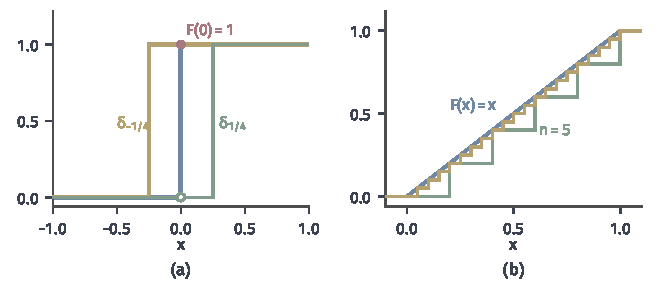
\includegraphics[width=112mm]{figures/07-probability/03-probability-limits/matplotlib/weak-cdf-criterion/figure.pdf}
 \caption{分布函数判据中的跳点。(a)蓝色为$\delta_0$的分布函数，绿色为$\delta_{1/4}$，黄色为$\delta_{-1/4}$；红点为$F(0)=1$，$\delta_{1/n}$在$0$处的值恒为$0$。(b)格点均匀分布$U_5$（绿色阶梯）与$U_{20}$（黄色阶梯）的分布函数，蓝线为$F(x)=x$。}
 \label{fig:weak-cdf-criterion}
\end{BookInlineFigure}

\paragraph{二项分布到Poisson分布}
现在可以把章首的现象写成定理。设$X_n\sim\operatorname{Bin}(n,2/n)$（$n\geq3$），$N\sim\operatorname{Poisson}(2)$。第~\ref{chap:common-distributions}章已经证明，对每个非负整数$k$，$\mathbb{P}(X_n=k)\to\mathbb{P}(N=k)$。分布函数在$x<0$时都为零；$x\geq0$时是有限和
\[
 F_n(x)=\sum_{k=0}^{\lfloor x\rfloor}\mathbb{P}(X_n=k)\longrightarrow\sum_{k=0}^{\lfloor x\rfloor}\mathbb{P}(N=k)=F(x) .
\]
所以$F_n(x)\to F(x)$对每个$x$成立，由定理~\ref{thm:weak-cdf-criterion}，$X_n\xrightarrow{\mathrm{d}}\operatorname{Poisson}(2)$。这里在跳点处也收敛；定理只是允许跳点处不收敛，并不要求它不收敛。

以$x=2$为例，$F(2)=5\mathrm{e}^{-2}\approx0.6767$，而
\[
 F_4(2)=0.6875,\qquad F_{10}(2)=0.6778,\qquad F_{40}(2)=0.6767 .
\]
图~\ref{fig:weak-binomial-poisson}(a)比较两个分布函数，(b)画出$\sup_x\lvert F_n(x)-F(x)\rvert$随$n$的变化，它大致按$1/n$缩小。弱收敛本身只断言极限，不给速度；这个速度是此例的具体计算结果。

\begin{BookInlineFigure}
 \centering
 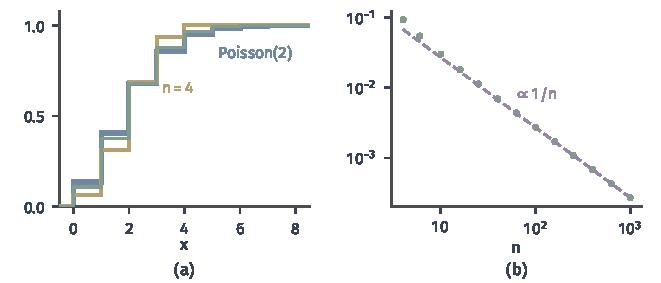
\includegraphics[width=112mm]{figures/07-probability/03-probability-limits/matplotlib/weak-binomial-poisson/figure.pdf}
 \caption{$\operatorname{Bin}(n,2/n)$向$\operatorname{Poisson}(2)$的弱收敛。(a)蓝色阶梯为$\operatorname{Poisson}(2)$的分布函数，黄色为$n=4$，绿色为$n=10$。(b)$\sup_x\lvert F_n(x)-F(x)\rvert$（绿点，对数坐标），紫色虚线是斜率为$-1$的参考线。}
 \label{fig:weak-binomial-poisson}
\end{BookInlineFigure}

分布函数判据还要求极限$F$本身是分布函数。若只知道$F_n$逐点收敛，极限可能不是分布函数：$\delta_n$的分布函数$\mathbf{1}_{\{x\geq n\}}$对每个$x$都趋于$0$。质量逃到了无穷远，下一节研究怎样防止这种情形。


\section{分布族的紧性}
\label{sec:weak-tightness}

前两节的判据都要先猜出极限分布，再去验证。很多时候极限并不知道，需要先判断一列分布有没有可能收敛到某个分布。实数列的情形可以作参照：有界数列不一定收敛，但总有收敛子列（Bolzano--Weierstrass定理）；无界数列可能连收敛子列都没有。分布列中扮演“无界”角色的，是概率质量逃向无穷远。

\paragraph{质量的逃逸}
$\delta_n$的全部质量跑到无穷远，分布函数对每个$x$都趋于$0$。逃逸也可以只是部分的。设$X_n\sim\mathcal{N}(0,n)$，则
\[
 F_n(x)=\Phi\bigl(x/\sqrt{n}\bigr)\longrightarrow\Phi(0)=\frac12,\qquad x\in\mathbb{R} .
\]
一半质量逃向$+\infty$，一半逃向$-\infty$，逐点极限是常数$1/2$，不是分布函数。再看$P_n=\frac12\delta_0+\frac12\delta_n$，它的分布函数趋于$\frac12\mathbf{1}_{\{x\geq0\}}$：留在原地的一半质量还在，跑远的一半消失了。图~\ref{fig:weak-mass-escape}画出这两种情形，它们都不可能弱收敛到任何概率分布。

\begin{BookInlineFigure}
 \centering
 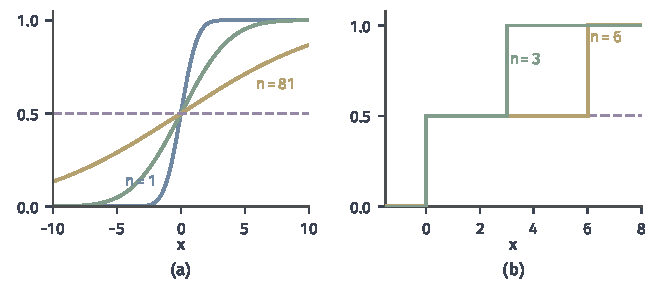
\includegraphics[width=112mm]{figures/07-probability/03-probability-limits/matplotlib/weak-mass-escape/figure.pdf}
 \caption{概率质量逃向无穷远。(a)$\mathcal{N}(0,n)$的分布函数，$n=1$（蓝）、$9$（绿）、$81$（黄），逐点趋于常数$1/2$（紫色虚线）。(b)$\frac12\delta_0+\frac12\delta_n$的分布函数，$n=3$（绿）与$n=6$（黄）；逐点极限$\frac12\mathbf{1}_{\{x\geq0\}}$（紫色虚线）的总质量只有$1/2$。}
 \label{fig:weak-mass-escape}
\end{BookInlineFigure}

\subsection{概率质量的控制}
\label{sec:weak-mass-control}

要防止逃逸，就要求所有分布在远处的质量能被同一个界控制。对单个分布这总能做到，因为$P(\lVert\bm{x}\rVert_2>r)$随$r\to\infty$趋于零；困难在于对一整族分布同时做到。

\begin{definition}[胎紧]
\label{def:weak-tight}
设$\{P_i\}_{i\in I}$是$\mathbb{R}^{d}$上的一族概率分布。若对每个$\varepsilon>0$，存在$r>0$使
\begin{equation}
 \sup_{i\in I}P_i\bigl(\{\bm{x}:\lVert\bm{x}\rVert_2>r\}\bigr)\leq\varepsilon ,
 \label{eq:weak-tight}
\end{equation}
则称这族分布\term{胎紧}（tight），也简称紧。一族随机向量称为胎紧，是指它们的分布胎紧。
\end{definition}

$\mathbb{R}^{d}$中有界闭集是紧集，所以式~\eqref{eq:weak-tight}也可以说成：存在紧集$K$，使每个$P_i$在$K$外的质量都不超过$\varepsilon$。单个分布胎紧；有限个胎紧族的并仍然胎紧，取各自的$r$中最大的一个即可。

直接验证式~\eqref{eq:weak-tight}往往不方便，矩的一致界给出常用的充分条件。

\begin{theorem}[矩的一致界蕴含胎紧]
\label{thm:weak-moment-tight}
设存在$p>0$与$M<\infty$，使$\mathbb{E}[\lVert\bm{X}_i\rVert_2^{p}]\leq M$对一切$i\in I$成立，则$\{\bm{X}_i\}_{i\in I}$胎紧，并且
\begin{equation}
 \sup_{i\in I}\mathbb{P}\bigl(\lVert\bm{X}_i\rVert_2>r\bigr)\leq\frac{M}{r^{p}},\qquad r>0 .
 \label{eq:weak-moment-tight}
\end{equation}
\end{theorem}

\begin{proof}
对非负变量$\lVert\bm{X}_i\rVert_2^{p}$用第~\ref{chap:tail-probabilities}章的Markov不等式，
\[
 \mathbb{P}\bigl(\lVert\bm{X}_i\rVert_2>r\bigr)\leq\mathbb{P}\bigl(\lVert\bm{X}_i\rVert_2^{p}\geq r^{p}\bigr)\leq\frac{M}{r^{p}} .
\]
取$r=(M/\varepsilon)^{1/p}$即得式~\eqref{eq:weak-tight}。
\end{proof}

对照前面的例子。$X_n\sim\operatorname{Bin}(n,2/n)$的期望恒为$2$，取$p=1$得$\mathbb{P}(X_n>r)\leq2/r$，胎紧。格点均匀分布都在$[0,1]$中，取$r=1$时式~\eqref{eq:weak-tight}左边为零。$\mathcal{N}(0,n)$的方差$n$没有一致界，它确实不胎紧：对任意固定的$r$，
\[
 \mathbb{P}(\lvert X_n\rvert>r)=2\bigl(1-\Phi(r/\sqrt{n})\bigr)\longrightarrow1 .
\]

\paragraph{胎紧与一致可积}
第~\ref{chap:random-variable-convergence}章的一致可积性也控制尾部，但控制的量不同。实随机变量族$\{X_i\}$一致可积，是指
\[
 \lim_{r\to\infty}\sup_{i\in I}\mathbb{E}\bigl[\lvert X_i\rvert\mathbf{1}_{\{\lvert X_i\rvert>r\}}\bigr]=0 .
\]
胎紧只数远处有多少质量；一致可积还要乘上质量所在的位置$\lvert x\rvert$，像力矩一样，远处的少量质量会被放大。在事件$\lvert X_i\rvert>r$上$\lvert X_i\rvert$至少是$r$，取期望得
\[
 \mathbb{P}\bigl(\lvert X_i\rvert>r\bigr)\leq\frac1r\,\mathbb{E}\bigl[\lvert X_i\rvert\mathbf{1}_{\{\lvert X_i\rvert>r\}}\bigr] ,
\]
所以一致可积蕴含胎紧。

反过来不成立。设$X_n$以概率$1/n$取$n$，以概率$1-1/n$取$0$。对$r\geq1$，只有$n>r$的那些$X_n$在$r$外有质量，质量为$1/n<1/r$，所以
\[
 \sup_{n}\mathbb{P}(X_n>r)\leq\frac1r,\qquad \sup_{n}\mathbb{E}\bigl[X_n\mathbf{1}_{\{X_n>r\}}\bigr]=\sup_{n>r}n\cdot\frac1n=1 .
\]
这族变量胎紧，却不一致可积。远处的质量$1/n$越来越少，而它与位置$n$的乘积始终是$1$。图~\ref{fig:weak-tight-vs-ui}对比了这两个量。第~\ref{sec:weak-integral-limits}节将看到，这个差别决定了期望能否随分布取极限。

\begin{BookInlineFigure}
 \centering
 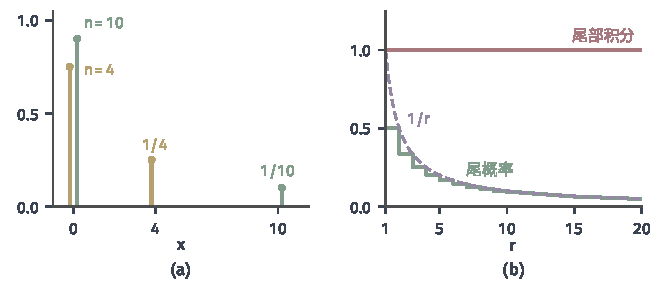
\includegraphics[width=112mm]{figures/07-probability/03-probability-limits/matplotlib/weak-tight-vs-ui/figure.pdf}
 \caption{胎紧与一致可积的差别，$X_n$以概率$1/n$取$n$，否则取$0$。(a)$n=4$（黄）与$n=10$（绿）的质量；远处质点很轻，乘以位置后都等于$1$。(b)作为$r$的函数，$\sup_n\mathbb{P}(X_n>r)$（绿）趋于零，紫色虚线为上界$1/r$；$\sup_n\mathbb{E}[X_n\mathbf{1}_{\{X_n>r\}}]$（红）恒为$1$。}
 \label{fig:weak-tight-vs-ui}
\end{BookInlineFigure}

\subsection{弱收敛子列}
\label{sec:weak-subsequences}

胎紧在分布列中的作用，正如有界性在实数列中的作用。下面的定理是Bolzano--Weierstrass定理的对应物。

\begin{theorem}[胎紧与弱收敛子列]
\label{thm:weak-prokhorov}
设$\{P_n\}$是$\mathbb{R}^{d}$上的概率分布列。
\begin{enumerate}
 \item 若$\{P_n\}$胎紧，则存在子列$P_{n_k}$与概率分布$P$，使$P_{n_k}\xrightarrow{\mathrm{w}}P$。
 \item 若一族分布中任取的序列都有弱收敛到概率分布的子列，则这族分布胎紧。
\end{enumerate}
\end{theorem}

后一条中的性质称为弱收敛意义下的相对紧。所以在$\mathbb{R}^{d}$中，胎紧与相对紧是同一回事。下面对$d=1$证明第一条，并对一般$d$证明第二条。

\begin{proof}
(1)，$d=1$。记$F_n$为$P_n$的分布函数，分四步。

第一步，用对角线方法在有理点上取收敛子列。把有理数排成$q_1,q_2,\dots$。数列$\bigl(F_n(q_1)\bigr)$在$[0,1]$中，有收敛子列；在这个子列中再取使$F_n(q_2)$收敛的子列，如此继续。取第$k$次所得子列的第$k$项，得到子列$(n_k)$，使对每个有理数$q$，$F_{n_k}(q)$收敛到某个$G(q)\in[0,1]$。$G$在有理数上不减。

第二步，构造右连续的极限。令
\[
 F(x)=\inf\{G(q):q\text{为有理数},\,q>x\} .
\]
$F$不减。若$x_m\downarrow x$，对每个有理数$q>x$，$m$足够大时$q>x_m$，于是$F(x_m)\leq G(q)$；对$q$取下确界得$\lim_mF(x_m)\leq F(x)$，而单调性给出反向不等式，所以$F$右连续。

第三步，在$F$的连续点$x$处证明$F_{n_k}(x)\to F(x)$。任取$\varepsilon>0$。由左连续性，取$y<x$使$F(y)>F(x)-\varepsilon$；由$F(x)$的定义，取有理数$s>x$使$G(s)<F(x)+\varepsilon$；再取有理数$r\in(y,x)$，由$F(y)$的定义有$F(y)\leq G(r)$。$F_{n_k}$不减，于是
\[
 \begin{aligned}
 \limsup_{k\to\infty}F_{n_k}(x)&\leq\lim_{k\to\infty}F_{n_k}(s)=G(s)<F(x)+\varepsilon,\\
 \liminf_{k\to\infty}F_{n_k}(x)&\geq\lim_{k\to\infty}F_{n_k}(r)=G(r)\geq F(y)>F(x)-\varepsilon .
 \end{aligned}
\]

第四步，用胎紧说明$F$是分布函数。对$\varepsilon>0$取式~\eqref{eq:weak-tight}中的$r$。对有理数$q>r$，$F_n(q)\geq1-\varepsilon$对一切$n$成立，所以$G(q)\geq1-\varepsilon$，从而$x\geq r$时$F(x)\geq1-\varepsilon$。对有理数$q<-r$，$F_n(q)\leq\varepsilon$，所以$x<q$时$F(x)\leq G(q)\leq\varepsilon$。因此$F(-\infty)=0$，$F(+\infty)=1$。不减、右连续且两端极限为$0$与$1$的函数是某个概率分布$P$的分布函数（第~\ref{chap:probability-spaces}章）。由定理~\ref{thm:weak-cdf-criterion}，$P_{n_k}\xrightarrow{\mathrm{w}}P$。

(2)，一般$d$。设这族分布不胎紧，则存在$\varepsilon>0$，对每个$m$都能在族中取到$P_m$，使$P_m(\lVert\bm{x}\rVert_2>m)>\varepsilon$。按假设，$(P_m)$有子列$P_{m_k}\xrightarrow{\mathrm{w}}P$。固定$r>0$，集合$\{\lVert\bm{x}\rVert_2\geq r\}$是闭集，当$m_k\geq r$时它包含$\{\lVert\bm{x}\rVert_2>m_k\}$。由Portmanteau定理的(3)，
\[
 P\bigl(\lVert\bm{x}\rVert_2\geq r\bigr)\geq\limsup_{k\to\infty}P_{m_k}\bigl(\lVert\bm{x}\rVert_2\geq r\bigr)\geq\varepsilon .
\]
这对每个$r$成立，与$P(\lVert\bm{x}\rVert_2\geq r)\to0$矛盾。
\end{proof}

第一步取出的极限$G$总存在，第四步之前的$F$也总能构造出来，胎紧只在第四步起作用。图~\ref{fig:weak-mass-escape}(b)就是缺了第四步的情形：前三步的构造给出$\frac12\mathbf{1}_{\{x\geq0\}}$，它右连续、不减，但$F(+\infty)=1/2$。$d>1$时第一条的证明思路相同，用多元分布函数在有理点上取对角线子列，细节较繁，可查阅~\scite{math-kallenberg2021probability}。

定理的第一条也称为\term{Helly选择定理}（Helly selection theorem）。在一般的完备可分度量空间上，胎紧（式~\eqref{eq:weak-tight}中的球换成紧集）与相对紧仍然等价，这就是\term{Prokhorov定理}（Prokhorov theorem）；空间的完备与可分保证单个分布胎紧，是相对紧推出胎紧所需的条件。本卷只在有限维空间中使用它。

\paragraph{子列极限的唯一性}
胎紧只保证有收敛子列，不保证整列收敛。$P_n$在$\delta_0$与$\delta_1$之间交替，所有质量都在$[0,1]$中，胎紧；偶数项与奇数项各自收敛，极限不同，整列不收敛。数列的情形也一样：有界数列收敛，当且仅当它所有收敛子列的极限相同。

\begin{lemma}[子列原则]
\label{lem:weak-subsequence}
设$\{P_n\}$胎紧，并且每个弱收敛的子列都收敛到同一个分布$P$，则$P_n\xrightarrow{\mathrm{w}}P$。
\end{lemma}

\begin{proof}
若不然，存在$f\in C_b(\mathbb{R}^{d})$、$\varepsilon>0$和子列$(n_k)$，使对一切$k$，
\[
 \Bigl\lvert\int f\,\mathrm{d}P_{n_k}-\int f\,\mathrm{d}P\Bigr\rvert\geq\varepsilon .
\]
子列仍胎紧，由定理~\ref{thm:weak-prokhorov}，它有进一步的子列弱收敛，按假设极限为$P$。沿这个进一步的子列，$\int f\,\mathrm{d}P_{n_k}\to\int f\,\mathrm{d}P$，与上式矛盾。
\end{proof}

这个引理把弱收敛的证明分成两件互相独立的事：用胎紧得到子列极限的存在，用别的办法证明子列极限只有一个。第~\ref{sec:weak-cf}节将用特征函数完成后一件事。


\section{特征函数}
\label{sec:weak-cf}

按定义验证弱收敛，要对每个有界连续函数检查读数，这在实际中无法做到。我们希望找一小族测试函数，它们由一个参数标记，同时满足三点：读数能确定分布；读数的收敛能推出弱收敛；独立变量相加时读数容易计算。复指数$\mathrm{e}^{\mathrm{i}tx}$正好满足这些要求。它的实部$\cos(tx)$与虚部$\sin(tx)$都有界连续；并且
\[
 \mathrm{e}^{\mathrm{i}t(x+y)}=\mathrm{e}^{\mathrm{i}tx}\,\mathrm{e}^{\mathrm{i}ty} ,
\]
加法变成了乘法。本节依次建立它的定义、运算、与矩的关系、对分布的识别，以及与弱收敛的联系。所需的Fourier分析都在概率对象上直接说明，不假定分布有密度。

\subsection{定义}
\label{sec:weak-cf-definition}

复值随机变量$Y_1+\mathrm{i}Y_2$的期望按实部、虚部分别取：
\[
 \mathbb{E}[Y_1+\mathrm{i}Y_2]=\mathbb{E}[Y_1]+\mathrm{i}\,\mathbb{E}[Y_2] .
\]
复值积分的性质可参考\BookChapterRef{chap:integration}{卷四第6章“积分”}，这里要用的是线性，以及期望的模不超过模的期望。

\begin{definition}[特征函数]
\label{def:weak-cf}
实随机变量$X$的\term{特征函数}（characteristic function）是
\begin{equation}
 \phi_X(t)=\mathbb{E}\bigl[\mathrm{e}^{\mathrm{i}tX}\bigr]=\mathbb{E}[\cos(tX)]+\mathrm{i}\,\mathbb{E}[\sin(tX)],\qquad t\in\mathbb{R} .
 \label{eq:weak-cf}
\end{equation}
取值于$\mathbb{R}^{d}$的随机向量$\bm{X}$的特征函数是
\begin{equation}
 \phi_{\bm{X}}(\bm{t})=\mathbb{E}\bigl[\mathrm{e}^{\mathrm{i}\langle\bm{t},\bm{X}\rangle}\bigr],\qquad \bm{t}\in\mathbb{R}^{d} .
 \label{eq:weak-cf-vector}
\end{equation}
\end{definition}

$\lvert\cos(tX)\rvert$与$\lvert\sin(tX)\rvert$都不超过$1$，所以特征函数对每个随机变量、每个$t$都存在，不需要任何矩条件。它只依赖$X$的分布，对分布$P$也写作$\phi_P$。

\paragraph{单位圆上的重心}
$\mathrm{e}^{\mathrm{i}tx}$是单位圆上辐角为$tx$的点。固定频率$t$，把取值$x$处的质量搬到单位圆上这个点，$\phi_X(t)$就是搬过去以后的重心。$t$很小时，各点挤在$1$附近，重心接近$1$；$t$变大，各点沿圆周散开，彼此抵消，重心向原点靠拢。所以$\lvert\phi_X(t)\rvert$描述分布在频率$t$下“转散”以后还剩多少一致性。

以均匀骰子为例，$X$在$\{1,\dots,6\}$上等可能取值，
\[
 \phi_X(t)=\frac16\sum_{k=1}^{6}\mathrm{e}^{\mathrm{i}tk} .
\]
$t=0.5$时，六个点散布在辐角$0.5$到$3$之间，重心约为$-0.120+0.661\mathrm{i}$，模约$0.672$。$t=\pi/3$时，六个点恰是正六边形的顶点，重心为$0$。图~\ref{fig:weak-cf-circle}画出这两个频率下的点与重心。

\begin{BookInlineFigure}
 \centering
 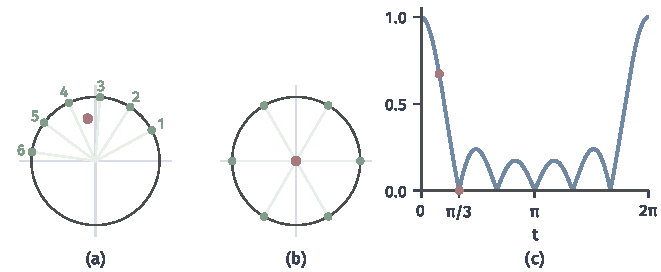
\includegraphics[width=112mm]{figures/07-probability/03-probability-limits/matplotlib/weak-cf-circle/figure.pdf}
 \caption{特征函数是单位圆上的重心。$X$为均匀骰子点数，绿点为$\mathrm{e}^{\mathrm{i}tk}$（$k=1,\dots,6$），每点质量$1/6$，红点为重心$\phi_X(t)$。(a)$t=0.5$；(b)$t=\pi/3$，六点构成正六边形，重心为$0$。(c)$\lvert\phi_X(t)\rvert$，$0\leq t\leq2\pi$，红点对应(a)(b)两个频率。}
 \label{fig:weak-cf-circle}
\end{BookInlineFigure}

\paragraph{基本性质}
由定义直接得到三条性质。第一，$\phi_X(0)=1$，且
\[
 \lvert\phi_X(t)\rvert\leq\mathbb{E}\bigl[\lvert\mathrm{e}^{\mathrm{i}tX}\rvert\bigr]=1 .
\]
第二，共轭对称：$\mathrm{e}^{-\mathrm{i}tX}$是$\mathrm{e}^{\mathrm{i}tX}$的共轭，所以$\phi_X(-t)=\overline{\phi_X(t)}$。若$X$与$-X$同分布，则$\phi_X(t)=\phi_{-X}(t)=\phi_X(-t)$，再由共轭对称，$\phi_X(t)$等于自己的共轭，特征函数是实的。

第三，一致连续。对任意$t$与$h$，
\[
 \lvert\phi_X(t+h)-\phi_X(t)\rvert=\bigl\lvert\mathbb{E}\bigl[\mathrm{e}^{\mathrm{i}tX}(\mathrm{e}^{\mathrm{i}hX}-1)\bigr]\bigr\rvert\leq\mathbb{E}\bigl[\lvert\mathrm{e}^{\mathrm{i}hX}-1\rvert\bigr] .
\]
右边不含$t$。$h\to0$时$\lvert\mathrm{e}^{\mathrm{i}hX}-1\rvert$逐点趋于零且不超过$2$，由支配收敛定理，右边趋于零。随机向量的情形完全相同。

\paragraph{常见分布}
离散分布按定义求和。$X\sim\operatorname{Bern}(p)$时，$\phi_X(t)=1-p+p\,\mathrm{e}^{\mathrm{i}t}$。$N\sim\operatorname{Poisson}(\lambda)$时，用指数函数的幂级数，
\[
 \phi_N(t)=\sum_{k\geq0}\mathrm{e}^{-\lambda}\frac{(\lambda\mathrm{e}^{\mathrm{i}t})^{k}}{k!}=\exp\bigl(\lambda(\mathrm{e}^{\mathrm{i}t}-1)\bigr) .
\]

有密度的分布按定义积分。$X\sim\operatorname{Unif}(-1,1)$时，虚部的被积函数是奇函数，积分为零，
\[
 \phi_X(t)=\frac12\int_{-1}^{1}\cos(tx)\,\mathrm{d}x=\frac{\sin t}{t},\qquad t\neq0 ,
\]
$\phi_X(0)=1$。

标准高斯$Z\sim\mathcal{N}(0,1)$的特征函数用一个微分方程求出。先说明可以在积分号下对$t$求导。对实数$a$，
\[
 \lvert\mathrm{e}^{\mathrm{i}a}-1\rvert=\Bigl\lvert\int_0^a\mathrm{i}\,\mathrm{e}^{\mathrm{i}s}\,\mathrm{d}s\Bigr\rvert\leq\lvert a\rvert .
\]
于是差商满足
\[
 \Bigl\lvert\mathrm{e}^{\mathrm{i}tx}\,\frac{\mathrm{e}^{\mathrm{i}hx}-1}{h}\,\varphi(x)\Bigr\rvert\leq\lvert x\rvert\varphi(x) .
\]
右边可积，由支配收敛定理，
\[
 \phi_Z'(t)=\int_{-\infty}^{\infty}\mathrm{i}x\,\mathrm{e}^{\mathrm{i}tx}\varphi(x)\,\mathrm{d}x .
\]

再用$x\varphi(x)=-\varphi'(x)$分部积分。边界项$\mathrm{e}^{\mathrm{i}tx}\varphi(x)$在$\pm\infty$处为零，于是
\[
 \phi_Z'(t)=-\mathrm{i}\int_{-\infty}^{\infty}\mathrm{e}^{\mathrm{i}tx}\varphi'(x)\,\mathrm{d}x=\mathrm{i}\int_{-\infty}^{\infty}\mathrm{i}t\,\mathrm{e}^{\mathrm{i}tx}\varphi(x)\,\mathrm{d}x=-t\,\phi_Z(t) .
\]
由此$\bigl(\mathrm{e}^{t^2/2}\phi_Z(t)\bigr)'=0$，结合$\phi_Z(0)=1$，得
\begin{equation}
 \phi_Z(t)=\mathrm{e}^{-t^2/2} .
 \label{eq:weak-gaussian-cf}
\end{equation}
标准高斯的特征函数与密度只差一个常数因子，这是后面高斯平滑论证的关键。

\subsection{变换与独立和}
\label{sec:weak-cf-operations}

先看确定的线性变换。对实数$a,b$，把$\mathrm{e}^{\mathrm{i}t(aX+b)}$拆成$\mathrm{e}^{\mathrm{i}tb}$与$\mathrm{e}^{\mathrm{i}(at)X}$之积，取期望得
\begin{equation}
 \phi_{aX+b}(t)=\mathrm{e}^{\mathrm{i}tb}\,\phi_X(at) .
 \label{eq:weak-cf-affine}
\end{equation}
平移只乘一个模为一的因子，不改变$\lvert\phi\rvert$；数乘$a$把频率轴伸缩$a$倍。对随机向量，设$\bm{A}$是$k\times d$矩阵，$\bm{b}\in\mathbb{R}^{k}$。由
\[
 \langle\bm{t},\bm{A}\bm{X}\rangle=\langle\bm{A}^{\top}\bm{t},\bm{X}\rangle ,
\]
得到
\begin{equation}
 \phi_{\bm{A}\bm{X}+\bm{b}}(\bm{t})=\mathrm{e}^{\mathrm{i}\langle\bm{t},\bm{b}\rangle}\,\phi_{\bm{X}}(\bm{A}^{\top}\bm{t}),\qquad\bm{t}\in\mathbb{R}^{k} .
 \label{eq:weak-cf-linear}
\end{equation}

例如$X\sim\mathcal{N}(\mu,\sigma^2)$可以写成$\mu+\sigma Z$，由式~\eqref{eq:weak-gaussian-cf}与式~\eqref{eq:weak-cf-affine}，
\[
 \phi_X(t)=\exp\Bigl(\mathrm{i}\mu t-\frac{\sigma^2t^2}{2}\Bigr) .
\]

\paragraph{独立和}
独立性把乘积的期望拆成期望的乘积，这正是复指数的加法性质需要的。

\begin{theorem}[独立和的特征函数]
\label{thm:weak-cf-independent}
设$\bm{X}$与$\bm{Y}$是相互独立、分别取值于$\mathbb{R}^{d}$与$\mathbb{R}^{k}$的随机向量。则联合特征函数可以分解为
\begin{equation}
 \phi_{(\bm{X},\bm{Y})}(\bm{s},\bm{t})=\phi_{\bm{X}}(\bm{s})\,\phi_{\bm{Y}}(\bm{t}),\qquad\bm{s}\in\mathbb{R}^{d},\ \bm{t}\in\mathbb{R}^{k} .
 \label{eq:weak-cf-joint-independent}
\end{equation}
特别地，$k=d$时，
\begin{equation}
 \phi_{\bm{X}+\bm{Y}}(\bm{t})=\phi_{\bm{X}}(\bm{t})\,\phi_{\bm{Y}}(\bm{t}) .
 \label{eq:weak-cf-sum}
\end{equation}
对相互独立的$\bm{X}_1,\dots,\bm{X}_n$，和的特征函数是$\prod_{j}\phi_{\bm{X}_j}$。
\end{theorem}

\begin{proof}
对有界可测的实函数$g,h$，独立性给出（第~\ref{chap:random-vectors}章）
\[
 \mathbb{E}[g(\bm{X})h(\bm{Y})]=\mathbb{E}[g(\bm{X})]\,\mathbb{E}[h(\bm{Y})] .
\]
把$\mathrm{e}^{\mathrm{i}\langle\bm{s},\bm{X}\rangle}$与$\mathrm{e}^{\mathrm{i}\langle\bm{t},\bm{Y}\rangle}$各自拆成实部与虚部，它们都是有界可测函数，乘开后有四项，每项都按上式分解，再合并，即得式~\eqref{eq:weak-cf-joint-independent}。取$\bm{s}=\bm{t}$，由内积的线性得式~\eqref{eq:weak-cf-sum}。$n$项的情形对$n$归纳。
\end{proof}

用已知分布检验这个公式。$\operatorname{Bin}(n,p)$是$n$个独立$\operatorname{Bern}(p)$之和，按式~\eqref{eq:weak-cf-sum}，
\[
 \phi(t)=\bigl(1-p+p\,\mathrm{e}^{\mathrm{i}t}\bigr)^{n} .
\]
按定义直接求和，由二项式定理，
\[
 \sum_{k=0}^{n}\binom nkp^{k}(1-p)^{n-k}\mathrm{e}^{\mathrm{i}tk}=\bigl(1-p+p\,\mathrm{e}^{\mathrm{i}t}\bigr)^{n} ,
\]
两者一致。独立的$\operatorname{Poisson}(\lambda_1)$与$\operatorname{Poisson}(\lambda_2)$之和，特征函数是$\exp\bigl((\lambda_1+\lambda_2)(\mathrm{e}^{\mathrm{i}t}-1)\bigr)$，正是$\operatorname{Poisson}(\lambda_1+\lambda_2)$的特征函数；下一小节的唯一性定理说明，和就服从这个分布。

多元高斯也可以这样算。设$\bm{Z}=(Z_1,\dots,Z_m)$的分量是独立的标准高斯变量，由式~\eqref{eq:weak-cf-joint-independent}，
\[
 \phi_{\bm{Z}}(\bm{s})=\prod_{j=1}^{m}\mathrm{e}^{-s_j^2/2}=\mathrm{e}^{-\lVert\bm{s}\rVert_2^2/2} .
\]
第~\ref{chap:multivariate-distributions}章把与$\bm{\mu}+\bm{A}\bm{Z}$同分布的随机向量$\bm{X}$定义为服从$\mathcal{N}(\bm{\mu},\bm{\Sigma})$，其中$\bm{\Sigma}=\bm{A}\bm{A}^{\top}$。由式~\eqref{eq:weak-cf-linear}，
\begin{equation}
 \phi_{\bm{X}}(\bm{t})=\exp\Bigl(\mathrm{i}\langle\bm{t},\bm{\mu}\rangle-\frac12\lVert\bm{A}^{\top}\bm{t}\rVert_2^2\Bigr)=\exp\Bigl(\mathrm{i}\langle\bm{t},\bm{\mu}\rangle-\frac12\bm{t}^{\top}\bm{\Sigma}\bm{t}\Bigr) .
 \label{eq:weak-mvn-cf}
\end{equation}
结果只通过$\bm{\Sigma}$依赖$\bm{A}$，与那一章的结论一致；$\bm{\Sigma}$奇异时公式照样成立。

\paragraph{没有独立时}
式~\eqref{eq:weak-cf-sum}离不开独立性。设$X\sim\operatorname{Unif}(-1,1)$，若$Y$是与$X$独立的同分布变量，$X+Y$的密度是$[-2,2]$上的三角形（第~\ref{chap:random-variable-transformations}章的卷积），特征函数是$(\sin t/t)^2$。若取$Y=X$，和是$2X$，由式~\eqref{eq:weak-cf-affine}，特征函数是$\sin(2t)/(2t)$。在$t=\pi/2$处，
\[
 \frac{\sin\pi}{\pi}=0,\qquad\Bigl(\frac{\sin(\pi/2)}{\pi/2}\Bigr)^{2}=\frac{4}{\pi^{2}}\approx0.405 ,
\]
两者不同。图~\ref{fig:weak-cf-sum}把两种和的密度与特征函数并排画出：边缘相同，配对方式不同，和的分布就不同。

\begin{BookInlineFigure}
 \centering
 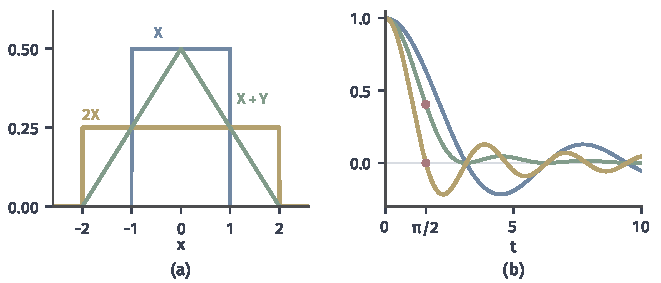
\includegraphics[width=112mm]{figures/07-probability/03-probability-limits/matplotlib/weak-cf-sum/figure.pdf}
 \caption{独立和与非独立和。(a)$\operatorname{Unif}(-1,1)$的密度（蓝），两个独立副本之和的三角形密度（绿），$2X$的均匀密度（黄）。(b)对应的特征函数$\sin t/t$、$(\sin t/t)^2$与$\sin(2t)/(2t)$，红点标出$t=\pi/2$处的两个值$4/\pi^2$与$0$。}
 \label{fig:weak-cf-sum}
\end{BookInlineFigure}

\subsection{矩与局部展开}
\label{sec:weak-cf-moments}

特征函数在原点附近的形状记录了矩。$\mathrm{e}^{\mathrm{i}tx}$对$t$求一次导数多出因子$\mathrm{i}x$，所以对期望求导，若能与期望交换，就得到$\mathbb{E}[\mathrm{i}X\mathrm{e}^{\mathrm{i}tX}]$。交换的条件是相应的绝对矩有限。为了控制余项，先给出复指数Taylor展开的误差界。

\begin{lemma}[复指数的展开误差]
\label{lem:weak-exp-remainder}
对实数$x$与整数$m\geq0$，
\begin{equation}
 \Bigl\lvert\mathrm{e}^{\mathrm{i}x}-\sum_{j=0}^{m}\frac{(\mathrm{i}x)^{j}}{j!}\Bigr\rvert\leq\min\Bigl(\frac{\lvert x\rvert^{m+1}}{(m+1)!},\ \frac{2\lvert x\rvert^{m}}{m!}\Bigr) .
 \label{eq:weak-exp-remainder}
\end{equation}
\end{lemma}

\begin{proof}
记左边绝对值内的量为$R_m(x)$。对$x$求导，
\[
 R_m'(x)=\mathrm{i}\,\mathrm{e}^{\mathrm{i}x}-\sum_{j=1}^{m}\frac{\mathrm{i}(\mathrm{i}x)^{j-1}}{(j-1)!}=\mathrm{i}R_{m-1}(x) ,
\]
又$R_m(0)=0$，所以$R_m(x)=\mathrm{i}\int_0^xR_{m-1}(s)\,\mathrm{d}s$。

对$m$归纳。$m=0$时，$R_0(x)=\mathrm{e}^{\mathrm{i}x}-1$，前面计算高斯特征函数时已经说明它的模不超过$\lvert x\rvert$；又由三角不等式，$\lvert R_0(x)\rvert\leq2$。设结论对$m-1$成立，则
\[
 \lvert R_m(x)\rvert\leq\int_0^{\lvert x\rvert}\min\Bigl(\frac{s^{m}}{m!},\frac{2s^{m-1}}{(m-1)!}\Bigr)\mathrm{d}s .
\]
分别只用最小值中的一项积分，得到$\lvert x\rvert^{m+1}/(m+1)!$与$2\lvert x\rvert^{m}/m!$两个上界。
\end{proof}

两个上界各有用处：$\lvert x\rvert$小时第一个更小，$\lvert x\rvert$大时第二个只增长到$m$次幂。下面的论证会同时用到这两种情形。

\begin{theorem}[矩与导数]
\label{thm:weak-cf-derivatives}
设$k\geq1$为整数，$\mathbb{E}[\lvert X\rvert^{k}]<\infty$。则$\phi_X$有直到$k$阶的连续导数，
\begin{equation}
 \phi_X^{(j)}(t)=\mathbb{E}\bigl[(\mathrm{i}X)^{j}\mathrm{e}^{\mathrm{i}tX}\bigr],\qquad
 \phi_X^{(j)}(0)=\mathrm{i}^{j}\,\mathbb{E}[X^{j}],\qquad j=0,1,\dots,k .
 \label{eq:weak-cf-derivatives}
\end{equation}
\end{theorem}

\begin{proof}
对$j$归纳，$j=0$即定义。设$j<k$时公式成立，考虑差商
\[
 \frac{\phi_X^{(j)}(t+h)-\phi_X^{(j)}(t)}{h}=\mathbb{E}\Bigl[(\mathrm{i}X)^{j}\mathrm{e}^{\mathrm{i}tX}\,\frac{\mathrm{e}^{\mathrm{i}hX}-1}{h}\Bigr] .
\]
由引理~\ref{lem:weak-exp-remainder}（$m=0$），期望内的量的模不超过$\lvert X\rvert^{j+1}$。$j+1\leq k$，且$\lvert X\rvert^{j+1}\leq1+\lvert X\rvert^{k}$，所以它可积。$h\to0$时期望内的量逐点趋于$(\mathrm{i}X)^{j+1}\mathrm{e}^{\mathrm{i}tX}$，由支配收敛定理得到$j+1$阶的公式。导数的连续性同样由支配收敛定理得到，控制函数是$\lvert X\rvert^{j}$。取$t=0$即得原点处的值。
\end{proof}

例如$N\sim\operatorname{Poisson}(2)$，它的特征函数已在第~\ref{sec:weak-cf-definition}节求出。逐次求导，
\[
 \begin{aligned}
 \phi_N'(t)&=2\mathrm{i}\,\mathrm{e}^{\mathrm{i}t}\phi_N(t),\\
 \phi_N''(t)&=\bigl((2\mathrm{i}\,\mathrm{e}^{\mathrm{i}t})^{2}-2\,\mathrm{e}^{\mathrm{i}t}\bigr)\phi_N(t) .
 \end{aligned}
\]
在原点，$\phi_N'(0)=2\mathrm{i}$，$\phi_N''(0)=-4-2=-6$。由式~\eqref{eq:weak-cf-derivatives}，
\[
 \mathbb{E}[N]=2,\qquad\mathbb{E}[N^{2}]=6,\qquad\operatorname{Var}(N)=6-4=2 ,
\]
与第~\ref{chap:common-distributions}章的结果相同。这里先由Poisson分布的各阶矩有限（其尾部比任何幂次都轻）保证求导合法，再读出矩。

\paragraph{二阶展开}
中心极限定理只需要原点附近到二阶的展开，而且只假定二阶矩有限。下面的定理给出展开和余项的控制。

\begin{theorem}[特征函数的二阶展开]
\label{thm:weak-cf-second-order}
设$\mathbb{E}[X^{2}]<\infty$。则
\begin{equation}
 \begin{gathered}
 \phi_X(t)=1+\mathrm{i}t\,\mathbb{E}[X]-\frac{t^{2}}{2}\mathbb{E}[X^{2}]+r(t),\\
 \lvert r(t)\rvert\leq t^{2}\,\mathbb{E}\Bigl[\min\Bigl(\frac{\lvert t\rvert\lvert X\rvert^{3}}{6},\,X^{2}\Bigr)\Bigr] ,
 \end{gathered}
 \label{eq:weak-cf-second-order}
\end{equation}
并且$r(t)/t^{2}\to0$（$t\to0$）。特别地，若$\mathbb{E}[X]=0$，$\operatorname{Var}(X)=\sigma^{2}$，则$\phi_X(t)=1-\sigma^{2}t^{2}/2+r(t)$。
\end{theorem}

\begin{proof}
在引理~\ref{lem:weak-exp-remainder}中取$m=2$，$x=tX$，
\[
 \Bigl\lvert\mathrm{e}^{\mathrm{i}tX}-1-\mathrm{i}tX+\frac{t^{2}X^{2}}{2}\Bigr\rvert\leq\min\Bigl(\frac{\lvert tX\rvert^{3}}{6},\,\lvert tX\rvert^{2}\Bigr)=t^{2}\min\Bigl(\frac{\lvert t\rvert\lvert X\rvert^{3}}{6},\,X^{2}\Bigr) .
\]
取期望，左边期望的模不小于$\lvert r(t)\rvert$，得到式~\eqref{eq:weak-cf-second-order}中的余项界。

$t\to0$时，对每个样本点，余项界中期望内的量不超过$\lvert t\rvert\lvert X\rvert^{3}/6$，因而趋于零；它又被可积的$X^{2}$控制。由支配收敛定理，余项界中的期望趋于零，即$r(t)/t^{2}\to0$。
\end{proof}

这里同时用了引理的两个上界。若只用$\lvert tX\rvert^{3}/6$，就需要三阶矩有限；$X^{2}$这一项让定理只依赖二阶矩，代价是只知道$r(t)=o(t^{2})$，不知道它以什么速度趋于零。

图~\ref{fig:weak-cf-local}比较三个均值为$0$、方差为$1$的分布：以$\pm1$各半取值的变量，特征函数为$\cos t$；$\operatorname{Unif}(-\sqrt3,\sqrt3)$，特征函数为$\sin(\sqrt3t)/(\sqrt3t)$；标准高斯$\mathrm{e}^{-t^{2}/2}$。三条曲线在原点附近都贴着抛物线$1-t^{2}/2$，离开原点后才分开。它们的四阶Taylor系数分别是$1/24$、$3/40$与$1/8$，正是四阶矩除以$4!$的不同。

\begin{BookInlineFigure}
 \centering
 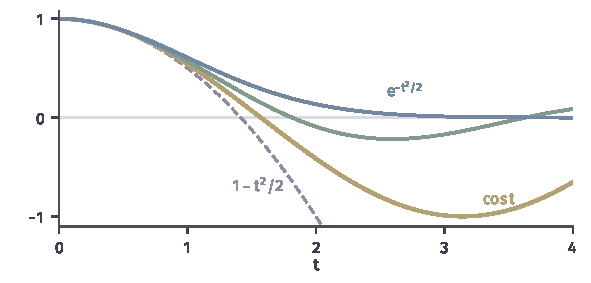
\includegraphics[width=100mm]{figures/07-probability/03-probability-limits/matplotlib/weak-cf-local/figure.pdf}
 \caption{特征函数的二阶展开。均值为$0$、方差为$1$的三个分布：$\pm1$各半（黄，$\cos t$），$\operatorname{Unif}(-\sqrt3,\sqrt3)$（绿），$\mathcal{N}(0,1)$（蓝）；紫色虚线为抛物线$1-t^{2}/2$。}
 \label{fig:weak-cf-local}
\end{BookInlineFigure}

\paragraph{不能反推的部分}
定理~\ref{thm:weak-cf-derivatives}从矩推出导数，反方向只部分成立。若$\phi_X$在原点有二阶导数，可以证明$\mathbb{E}[X^{2}]<\infty$；一般地，原点处存在$2k$阶导数蕴含$2k$阶矩有限。奇数阶则不然：存在对称分布，其特征函数在原点可导，期望$\mathbb{E}[\lvert X\rvert]$却是无穷大，例如尾部$\mathbb{P}(\lvert X\rvert>x)$像$1/(x\ln x)$那样衰减的分布。这些结论的证明可查阅~\scite{math-kallenberg2021probability}。因此，看到特征函数有若干阶导数，不能直接断言对应各阶矩都存在，更不能断言所有矩存在。

\subsection{分布唯一性}
\label{sec:weak-cf-uniqueness}

特征函数要作识别工具，首先必须做到：不同分布的特征函数不同。若分布有可积的密度，这是Fourier变换的单射性；但一般分布可能有原子，也可能既无原子又无密度。办法是先给分布加一点高斯噪声，把它抹成有光滑密度的分布，再让噪声趋于零。

\paragraph{高斯平滑}
平滑要用到高斯密度与其特征函数的对偶。取$\sigma>0$，考虑高斯分布$\mathcal{N}(\bm{0},\sigma^{-2}\bm{I}_d)$，它的密度是
\[
 \Bigl(\frac{\sigma^{2}}{2\pi}\Bigr)^{d/2}\mathrm{e}^{-\sigma^{2}\lVert\bm{s}\rVert_2^{2}/2},\qquad\bm{s}\in\mathbb{R}^{d} .
\]
由式~\eqref{eq:weak-mvn-cf}，它在$\bm{u}$处的特征函数是$\mathrm{e}^{-\lVert\bm{u}\rVert_2^{2}/(2\sigma^{2})}$。把特征函数写成积分，两边乘以常数$(2\pi\sigma^{2})^{-d/2}$，得到
\begin{equation}
 \begin{aligned}
 \frac{1}{(2\pi\sigma^{2})^{d/2}}\mathrm{e}^{-\lVert\bm{u}\rVert_2^{2}/(2\sigma^{2})}
 &=\frac{1}{(2\pi)^{d}}\int_{\mathbb{R}^{d}}\mathrm{e}^{\mathrm{i}\langle\bm{s},\bm{u}\rangle}\mathrm{e}^{-\sigma^{2}\lVert\bm{s}\rVert_2^{2}/2}\,\mathrm{d}\bm{s} .
 \end{aligned}
 \label{eq:weak-gauss-identity}
\end{equation}
左边是$\mathcal{N}(\bm{0},\sigma^{2}\bm{I}_d)$的密度，记作$g_{\sigma}(\bm{u})$。式~\eqref{eq:weak-gauss-identity}把它写成了复指数的叠加。

设$\bm{Z}\sim\mathcal{N}(\bm{0},\bm{I}_d)$与$\bm{X}$独立（必要时在乘积空间上构造）。给定$\bm{X}=\bm{x}_0$，$\bm{X}+\sigma\bm{Z}$服从以$\bm{x}_0$为中心的$\mathcal{N}(\bm{x}_0,\sigma^{2}\bm{I}_d)$。由独立性与Tonelli定理，对每个Borel集$A$，
\[
 \mathbb{P}(\bm{X}+\sigma\bm{Z}\in A)=\mathbb{E}\Bigl[\int_Ag_{\sigma}(\bm{x}-\bm{X})\,\mathrm{d}\bm{x}\Bigr]=\int_A\mathbb{E}\bigl[g_{\sigma}(\bm{x}-\bm{X})\bigr]\,\mathrm{d}\bm{x} .
\]
所以$\bm{X}+\sigma\bm{Z}$有密度
\[
 f_{\sigma}(\bm{x})=\mathbb{E}\bigl[g_{\sigma}(\bm{x}-\bm{X})\bigr] ,
\]
这就是把$\bm{X}$的每一份质量用一个小高斯“抹开”后的结果。

把式~\eqref{eq:weak-gauss-identity}代入$f_{\sigma}$，并交换期望与积分。被积函数的模不超过$\mathrm{e}^{-\sigma^{2}\lVert\bm{s}\rVert_2^{2}/2}$，它在乘积空间上可积，Fubini定理适用。于是
\begin{equation}
 f_{\sigma}(\bm{x})=\frac{1}{(2\pi)^{d}}\int_{\mathbb{R}^{d}}\mathrm{e}^{\mathrm{i}\langle\bm{s},\bm{x}\rangle}\,\phi_{\bm{X}}(-\bm{s})\,\mathrm{e}^{-\sigma^{2}\lVert\bm{s}\rVert_2^{2}/2}\,\mathrm{d}\bm{s} .
 \label{eq:weak-smoothed-density}
\end{equation}
平滑后的密度完全由特征函数算出。

\begin{theorem}[特征函数确定分布]
\label{thm:weak-cf-uniqueness}
设$\bm{X}$与$\bm{Y}$是取值于$\mathbb{R}^{d}$的随机向量。若$\phi_{\bm{X}}(\bm{t})=\phi_{\bm{Y}}(\bm{t})$对一切$\bm{t}\in\mathbb{R}^{d}$成立，则$P_{\bm{X}}=P_{\bm{Y}}$。
\end{theorem}

\begin{proof}
取$\bm{Z}$与$\bm{X}$独立，$\bm{Z}'$与$\bm{Y}$独立，都服从$\mathcal{N}(\bm{0},\bm{I}_d)$。由式~\eqref{eq:weak-smoothed-density}，对每个$\sigma>0$，$\bm{X}+\sigma\bm{Z}$与$\bm{Y}+\sigma\bm{Z}'$的密度相同，因而分布相同。

取$\sigma=1/m$。对每个样本点，$\bm{X}+\bm{Z}/m\to\bm{X}$，所以依概率收敛，由定理~\ref{thm:weak-prob-implies-dist}也依分布收敛；同样$\bm{Y}+\bm{Z}'/m\xrightarrow{\mathrm{d}}\bm{Y}$。两列随机向量的分布逐项相同，是同一个分布列，它同时弱收敛到$P_{\bm{X}}$与$P_{\bm{Y}}$。由引理~\ref{lem:weak-uniqueness}，$P_{\bm{X}}=P_{\bm{Y}}$。
\end{proof}

证明只用了弱收敛的定义、依概率收敛与依分布收敛的关系，以及极限唯一性，没有用到联合分布的极限判据。图~\ref{fig:weak-gaussian-smoothing}显示了平滑与还原：$\operatorname{Poisson}(2)$只有原子，没有密度；式~\eqref{eq:weak-smoothed-density}算出的$f_\sigma$在每个原子处鼓起一个小包，$\sigma$越小，小包越窄越高，质量越来越集中到原子上。

\begin{BookInlineFigure}
 \centering
 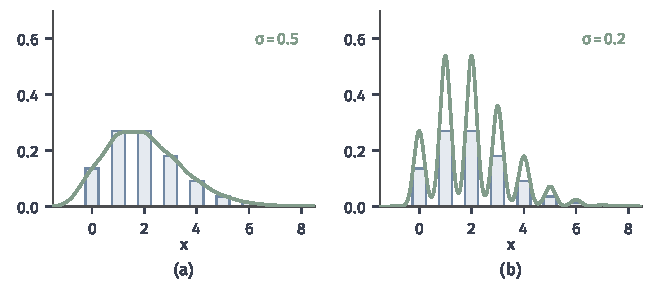
\includegraphics[width=112mm]{figures/07-probability/03-probability-limits/matplotlib/weak-gaussian-smoothing/figure.pdf}
 \caption{高斯平滑。浅蓝柱为$\operatorname{Poisson}(2)$在$k=0,\dots,7$的质量。曲线是由式~\eqref{eq:weak-smoothed-density}对特征函数数值积分得到的平滑密度$f_\sigma$：(a)$\sigma=0.5$（绿）；(b)$\sigma=0.2$（绿）。脚本同时按“各原子处放一个高斯小包”直接计算并核对两种结果相同。}
 \label{fig:weak-gaussian-smoothing}
\end{BookInlineFigure}

\paragraph{反演公式}
若$\phi_{\bm{X}}$本身在$\mathbb{R}^{d}$上可积，可以在式~\eqref{eq:weak-smoothed-density}中直接令$\sigma\to0$：被积函数被可积的$\lvert\phi_{\bm{X}}\rvert$控制，由支配收敛定理，$f_\sigma$一致收敛到
\begin{equation}
 f(\bm{x})=\frac{1}{(2\pi)^{d}}\int_{\mathbb{R}^{d}}\mathrm{e}^{-\mathrm{i}\langle\bm{t},\bm{x}\rangle}\,\phi_{\bm{X}}(\bm{t})\,\mathrm{d}\bm{t}
 \label{eq:weak-inversion}
\end{equation}
（积分变量换成了$\bm{t}=-\bm{s}$），这就是\term{反演公式}（inversion formula）。对连续且支撑有界的函数$h$，一方面$\mathbb{E}[h(\bm{X}+\sigma\bm{Z})]$等于$\int hf_\sigma$，趋于$\int hf$；另一方面由定理~\ref{thm:weak-prob-implies-dist}，它趋于$\mathbb{E}[h(\bm{X})]$。用这样的$h$从上方逼近闭长方体的示性函数，与引理~\ref{lem:weak-uniqueness}同样的单调极限说明，$\bm{X}$有连续密度$f$。这与\BookChapterRef{chap:fourier-transform}{卷四第14章“Fourier变换”}的$L^{1}$反演定理是同一件事，那里的约定在指数中带有$2\pi$，常数因而不同。

用反演公式可以求出一个不易直接积分的特征函数。$\operatorname{Laplace}(0,1)$的密度为$\frac12\mathrm{e}^{-\lvert x\rvert}$，它对称，特征函数为
\[
 \int_0^{\infty}\mathrm{e}^{-x}\cos(tx)\,\mathrm{d}x=\frac{1}{1+t^{2}} .
\]
它可积，由式~\eqref{eq:weak-inversion}，
\[
 \frac12\mathrm{e}^{-\lvert x\rvert}=\frac{1}{2\pi}\int_{-\infty}^{\infty}\frac{\mathrm{e}^{-\mathrm{i}tx}}{1+t^{2}}\,\mathrm{d}t .
\]
交换$x$与$t$的名字，两边乘以$2$。右边的被积函数中，Cauchy密度对称，$\mathrm{e}^{-\mathrm{i}tx}$可以换成$\mathrm{e}^{\mathrm{i}tx}$，于是右边就是标准Cauchy分布（密度$1/(\pi(1+x^{2}))$）在$t$处的特征函数，它等于$\mathrm{e}^{-\lvert t\rvert}$。

Cauchy分布的特征函数在原点不可导，与它没有期望相符。它还说明式~\eqref{eq:weak-cf-sum}的逆命题不成立：设$X$服从标准Cauchy分布，取$Y=X$，则
\[
 \phi_{X+Y}(t)=\phi_X(2t)=\mathrm{e}^{-2\lvert t\rvert}=\phi_X(t)\,\phi_Y(t) ,
\]
乘积公式成立，而$X$与$Y$并不独立。

\paragraph{有界变量的矩}
第~\ref{chap:random-variable-moments}章提到，取值有界时全部矩决定分布。现在可以证明这一点。设$\lvert X\rvert\leq M$，在引理~\ref{lem:weak-exp-remainder}中取$x=tX$并取期望，
\[
 \Bigl\lvert\phi_X(t)-\sum_{j=0}^{m}\frac{(\mathrm{i}t)^{j}}{j!}\mathbb{E}[X^{j}]\Bigr\rvert\leq\frac{(\lvert t\rvert M)^{m+1}}{(m+1)!}\longrightarrow0\qquad(m\to\infty) .
\]
所以对每个$t$，
\[
 \phi_X(t)=\sum_{j\geq0}\frac{(\mathrm{i}t)^{j}}{j!}\mathbb{E}[X^{j}] .
\]
两个有界变量若各阶矩相同，特征函数就相同，由定理~\ref{thm:weak-cf-uniqueness}，分布也相同。第~\ref{sec:weak-mgf}节将把有界的条件放宽为指数矩有限，并看到不加条件时结论可能失败。

\subsection{连续性定理}
\label{sec:weak-cf-continuity}

现在回到弱收敛。$\cos\langle\bm{t},\bm{x}\rangle$与$\sin\langle\bm{t},\bm{x}\rangle$是有界连续函数，所以弱收敛时特征函数逐点收敛。反过来，若特征函数逐点收敛，分布是否弱收敛？还要排除质量逃逸。

先看反例。$X_n\sim\mathcal{N}(0,n)$的特征函数是$\mathrm{e}^{-nt^{2}/2}$，它在$t=0$处恒为$1$，在$t\neq0$处趋于$0$。逐点极限
\[
 \psi(t)=\begin{cases}1,&t=0,\\0,&t\neq0\end{cases}
\]
存在，但在原点不连续；而第~\ref{sec:weak-tightness}节已经看到，这列分布的质量逃向无穷远，没有弱极限。原点附近的特征函数对应低频，也就是大尺度的形状；质量跑远，正表现为低频部分的塌缩。下面的引理把这个直观写成不等式。

\begin{lemma}[由特征函数控制尾概率]
\label{lem:weak-cf-tail}
设$X$是实随机变量，$u>0$，则
\begin{equation}
 \mathbb{P}\bigl(\lvert X\rvert\geq2/u\bigr)\leq\frac1u\int_{-u}^{u}\bigl(1-\phi_X(t)\bigr)\,\mathrm{d}t .
 \label{eq:weak-cf-tail}
\end{equation}
右边是实数，因为$\phi_X$的虚部是奇函数，积分为零。
\end{lemma}

\begin{proof}
对固定的$x\neq0$，
\[
 \frac1u\int_{-u}^{u}\bigl(1-\mathrm{e}^{\mathrm{i}tx}\bigr)\,\mathrm{d}t=2-\frac{2\sin(ux)}{ux}=2\Bigl(1-\frac{\sin(ux)}{ux}\Bigr) ,
\]
$x=0$时左边为$0$。被积函数有界，由Fubini定理交换期望与积分，
\[
 \frac1u\int_{-u}^{u}\bigl(1-\phi_X(t)\bigr)\,\mathrm{d}t=2\,\mathbb{E}\Bigl[1-\frac{\sin(uX)}{uX}\Bigr] ,
\]
其中$uX=0$时方括号内取$0$。

对一切实数$y\neq0$有$\lvert\sin y/y\rvert\leq1$，所以$1-\sin y/y\geq0$；当$\lvert y\rvert\geq2$时$\lvert\sin y/y\rvert\leq1/\lvert y\rvert\leq1/2$，所以$1-\sin y/y\geq1/2$。于是
\[
 2\,\mathbb{E}\Bigl[1-\frac{\sin(uX)}{uX}\Bigr]\geq2\cdot\frac12\,\mathbb{P}\bigl(\lvert uX\rvert\geq2\bigr)=\mathbb{P}\bigl(\lvert X\rvert\geq2/u\bigr) .
\]
\end{proof}

\begin{theorem}[连续性定理]
\label{thm:weak-continuity}
设$P_n$是$\mathbb{R}^{d}$上的概率分布，特征函数为$\phi_n$。
\begin{enumerate}
 \item 若$P_n\xrightarrow{\mathrm{w}}P$，则$\phi_n(\bm{t})\to\phi_P(\bm{t})$对每个$\bm{t}$成立。
 \item 若$\phi_n(\bm{t})$对每个$\bm{t}$收敛到某个$\psi(\bm{t})$，并且$\psi$在$\bm{0}$处连续，则存在概率分布$P$，使$\psi=\phi_P$且$P_n\xrightarrow{\mathrm{w}}P$。
\end{enumerate}
\end{theorem}

\begin{proof}
(1)：对固定的$\bm{t}$，$\phi_n(\bm{t})$的实部与虚部是有界连续函数$\cos\langle\bm{t},\bm{x}\rangle$与$\sin\langle\bm{t},\bm{x}\rangle$的读数，由定义~\ref{def:weak-convergence}收敛。

(2)：分两步。第一步证明$\{P_n\}$胎紧，先看$d=1$。$\psi(0)=\lim\phi_n(0)=1$。任取$\varepsilon>0$，由$\psi$在原点连续，取$u>0$使$\lvert1-\psi(t)\rvert\leq\varepsilon/2$对$\lvert t\rvert\leq u$成立，于是
\[
 \Bigl\lvert\frac1u\int_{-u}^{u}\bigl(1-\psi(t)\bigr)\,\mathrm{d}t\Bigr\rvert\leq\varepsilon .
\]
$\lvert1-\phi_n\rvert\leq2$，由支配收敛定理，
\[
 \frac1u\int_{-u}^{u}\bigl(1-\phi_n(t)\bigr)\,\mathrm{d}t\longrightarrow\frac1u\int_{-u}^{u}\bigl(1-\psi(t)\bigr)\,\mathrm{d}t .
\]
所以存在$N$，当$n\geq N$时左边小于$2\varepsilon$，由引理~\ref{lem:weak-cf-tail}，
\[
 P_n\bigl(\lvert x\rvert\geq2/u\bigr)<2\varepsilon,\qquad n\geq N .
\]
前$N-1$个分布各自胎紧，与之合并，整列胎紧。

$d>1$时，第$j$个坐标$x_j=\langle\bm{e}_j,\bm{x}\rangle$在$P_n$下的特征函数是$s\mapsto\phi_n(s\bm{e}_j)$，它逐点趋于$s\mapsto\psi(s\bm{e}_j)$，后者在$0$处连续。由一维的结论，每个坐标的分布胎紧。再由
\[
 P_n\bigl(\lVert\bm{x}\rVert_2>r\bigr)\leq\sum_{j=1}^{d}P_n\bigl(\lvert x_j\rvert>r/\sqrt{d}\bigr) ,
\]
$\{P_n\}$胎紧。

第二步识别极限。由定理~\ref{thm:weak-prokhorov}，$\{P_n\}$的每个子列都有进一步的子列弱收敛。设某个子列$P_{n_k}\xrightarrow{\mathrm{w}}Q$，由(1)，$\phi_Q=\lim\phi_{n_k}=\psi$。所以每个子列极限的特征函数都是$\psi$，由定理~\ref{thm:weak-cf-uniqueness}，它们是同一个分布，记作$P$。由引理~\ref{lem:weak-subsequence}，$P_n\xrightarrow{\mathrm{w}}P$，并且$\phi_P=\psi$。
\end{proof}

定理~\ref{thm:weak-continuity}常称为\term{Lévy连续性定理}（Lévy continuity theorem）。(2)的两步对应第~\ref{sec:weak-tightness}节末尾所说的两件事。原点连续性只用在第一步：它通过引理~\ref{lem:weak-cf-tail}保证质量不逃逸。识别极限则交给唯一性定理。结论中$\psi$是特征函数这一点也是证明的产物，并不需要事先知道。

\paragraph{再看二项分布到Poisson分布}
用连续性定理可以不经质量表重新证明$\operatorname{Bin}(n,2/n)\xrightarrow{\mathrm{w}}\operatorname{Poisson}(2)$。需要一个比较乘积的引理，它在下一章的中心极限定理中也要用到。

\begin{lemma}[乘积之差]
\label{lem:weak-product-difference}
设复数$a_1,\dots,a_n$与$b_1,\dots,b_n$的模都不超过$1$，则
\begin{equation}
 \Bigl\lvert\prod_{j=1}^{n}a_j-\prod_{j=1}^{n}b_j\Bigr\rvert\leq\sum_{j=1}^{n}\lvert a_j-b_j\rvert .
 \label{eq:weak-product-difference}
\end{equation}
\end{lemma}

\begin{proof}
$n=1$时是等式。设$n-1$时成立，把差拆成两部分：
\[
 \prod_{j=1}^{n}a_j-\prod_{j=1}^{n}b_j=a_n\Bigl(\prod_{j<n}a_j-\prod_{j<n}b_j\Bigr)+(a_n-b_n)\prod_{j<n}b_j .
\]
$\lvert a_n\rvert\leq1$，$\lvert\prod_{j<n}b_j\rvert\leq1$，由三角不等式与归纳假设即得。
\end{proof}

设$X_n\sim\operatorname{Bin}(n,2/n)$，记$z=2(\mathrm{e}^{\mathrm{i}t}-1)$，则
\[
 \phi_{X_n}(t)=\Bigl(1+\frac zn\Bigr)^{n},\qquad\exp\bigl(2(\mathrm{e}^{\mathrm{i}t}-1)\bigr)=\bigl(\mathrm{e}^{z/n}\bigr)^{n} .
\]
$n\geq2$时，$1+z/n=(1-2/n)+(2/n)\mathrm{e}^{\mathrm{i}t}$是单位圆盘中两点的凸组合，模不超过$1$；$z$的实部$2(\cos t-1)\leq0$，所以$\lvert\mathrm{e}^{z/n}\rvert\leq1$。

由引理~\ref{lem:weak-product-difference}，
\[
 \bigl\lvert\phi_{X_n}(t)-\mathrm{e}^{z}\bigr\rvert\leq n\,\Bigl\lvert1+\frac zn-\mathrm{e}^{z/n}\Bigr\rvert .
\]
对$\lvert w\rvert\leq1$，由幂级数，
\[
 \lvert\mathrm{e}^{w}-1-w\rvert\leq\sum_{k\geq2}\frac{\lvert w\rvert^{k}}{k!}\leq\lvert w\rvert^{2}(\mathrm{e}-2)\leq\lvert w\rvert^{2} .
\]
$\lvert z\rvert\leq4$，取$n\geq4$与$w=z/n$，得到
\[
 \bigl\lvert\phi_{X_n}(t)-\exp\bigl(2(\mathrm{e}^{\mathrm{i}t}-1)\bigr)\bigr\rvert\leq n\cdot\frac{\lvert z\rvert^{2}}{n^{2}}\leq\frac{16}{n} .
\]
所以特征函数收敛到$\operatorname{Poisson}(2)$的特征函数，后者连续，由连续性定理即得弱收敛。

以$t=\pi$为例，$z=-4$，$\phi_{X_n}(\pi)=(1-4/n)^{n}$。$n=10$与$n=40$时依次为
\[
 0.6^{10}\approx0.00605,\qquad0.9^{40}\approx0.0148 ,
\]
极限为$\mathrm{e}^{-4}\approx0.0183$。图~\ref{fig:weak-continuity}(a)画出特征函数实部的收敛；(b)是$\mathcal{N}(0,n)$的反例，极限在原点断开。

\begin{BookInlineFigure}
 \centering
 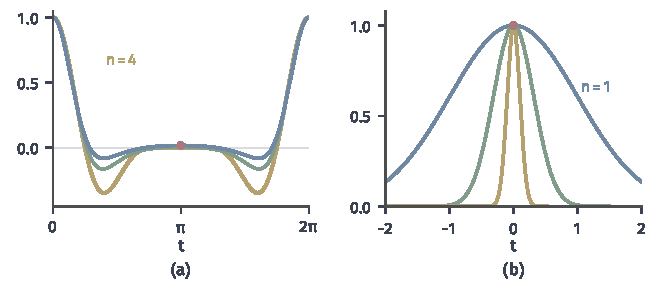
\includegraphics[width=112mm]{figures/07-probability/03-probability-limits/matplotlib/weak-continuity/figure.pdf}
 \caption{连续性定理的两种情形。(a)$\operatorname{Bin}(n,2/n)$特征函数的实部，$n=4$（黄）、$10$（绿），蓝线为$\operatorname{Poisson}(2)$的$\operatorname{Re}\exp(2(\mathrm{e}^{\mathrm{i}t}-1))$，红点为$t=\pi$处的极限$\mathrm{e}^{-4}$。(b)$\mathcal{N}(0,n)$的特征函数$\mathrm{e}^{-nt^2/2}$，$n=1$（蓝）、$10$（绿）、$100$（黄），逐点极限在原点为$1$（红点）、其余为$0$。}
 \label{fig:weak-continuity}
\end{BookInlineFigure}


\section{矩母函数}
\label{sec:weak-mgf}

第~\ref{chap:tail-probabilities}章用矩母函数$M_X(t)=\mathbb{E}[\mathrm{e}^{tX}]$给出尾概率的指数界，并提到它在一定条件下决定分布。它与特征函数只差一个$\mathrm{i}$：把$\mathrm{e}^{\mathrm{i}tX}$换成$\mathrm{e}^{tX}$。可是这一换，被积函数不再有界，$M_X(t)$可能是$+\infty$。本节研究它在哪里有限，有限时能做什么，以及它与特征函数的分工。

\paragraph{有限的范围}
记$D_X=\{t\in\mathbb{R}:M_X(t)<\infty\}$。总有$0\in D_X$。$D_X$是一个区间：若$t_1,t_2\in D_X$，$0<\theta<1$，由$t\mapsto\mathrm{e}^{tx}$的凸性，
\[
 \mathrm{e}^{(\theta t_1+(1-\theta)t_2)x}\leq\theta\,\mathrm{e}^{t_1x}+(1-\theta)\,\mathrm{e}^{t_2x} ,
\]
取期望知$\theta t_1+(1-\theta)t_2\in D_X$。这个区间可以是整条实轴、半直线、有界区间，也可以只有一个点。

几个例子。$\mathcal{N}(0,1)$与$\operatorname{Poisson}(\lambda)$的矩母函数分别是$\mathrm{e}^{t^{2}/2}$与$\exp(\lambda(\mathrm{e}^{t}-1))$，对一切$t$有限。$\operatorname{Exp}(1)$的矩母函数是$1/(1-t)$，$D_X=(-\infty,1)$。标准Cauchy分布的密度只按$x^{-2}$衰减，$t\neq0$时$\mathrm{e}^{tx}$在一侧指数增长，积分发散，$D_X=\{0\}$。$D_X$能否包含$0$的一个邻域，取决于两侧尾部是否都至少按指数衰减。

\paragraph{生成矩}
在$0$的邻域上有限时，矩母函数配得上它的名字。

\begin{theorem}[矩母函数与矩]
\label{thm:weak-mgf-moments}
设存在$t_0>0$，使$M_X(t)<\infty$对$\lvert t\rvert<t_0$成立。则
\begin{enumerate}
 \item 对每个整数$k\geq0$与$0<t<t_0$，
 \begin{equation}
 \mathbb{E}\bigl[\lvert X\rvert^{k}\bigr]\leq\frac{k!}{t^{k}}\bigl(M_X(t)+M_X(-t)\bigr)<\infty ;
 \label{eq:weak-mgf-moment-bound}
 \end{equation}
 \item 对$\lvert t\rvert<t_0$，$M_X(t)=\sum_{k\geq0}t^{k}\,\mathbb{E}[X^{k}]/k!$；
 \item $M_X$在$(-t_0,t_0)$上任意次可导，$M_X^{(k)}(0)=\mathbb{E}[X^{k}]$。
\end{enumerate}
\end{theorem}

\begin{proof}
(1)：对$t>0$，$\mathrm{e}^{t\lvert x\rvert}$的幂级数每一项非负，保留第$k$项，得
\[
 \frac{t^{k}\lvert x\rvert^{k}}{k!}\leq\mathrm{e}^{t\lvert x\rvert}\leq\mathrm{e}^{tx}+\mathrm{e}^{-tx} ,
\]
第二个不等号是因为$\mathrm{e}^{t\lvert x\rvert}$就是$\mathrm{e}^{tx}$与$\mathrm{e}^{-tx}$中较大的一个。代入$X$并取期望即得。

(2)：部分和满足
\[
 \Bigl\lvert\sum_{k=0}^{m}\frac{(tX)^{k}}{k!}\Bigr\rvert\leq\mathrm{e}^{\lvert t\rvert\lvert X\rvert}\leq\mathrm{e}^{tX}+\mathrm{e}^{-tX} ,
\]
右边可积，部分和逐点趋于$\mathrm{e}^{tX}$。由支配收敛定理，期望与求和可以交换。

(3)：由(2)，$M_X$在$(-t_0,t_0)$上是收敛的幂级数，可以逐项求导任意次（可参考\BookChapterRef{chap:univariate-differentiation}{卷一第6章“一元函数的微分”}），$t^{k}$的系数乘以$k!$就是$k$阶导数在$0$处的值。
\end{proof}

这回答了第~\ref{chap:tail-probabilities}章留下的问题：逐项取期望的依据是支配收敛定理，控制函数是$\mathrm{e}^{tX}+\mathrm{e}^{-tX}$，它的可积性正来自$0$两侧的有限性。例如$X\sim\operatorname{Exp}(1)$，$1/(1-t)=\sum_{k\geq0}t^{k}$对$\lvert t\rvert<1$成立，比较系数得
\[
 \mathbb{E}[X^{k}]=k!,\qquad k=0,1,2,\dots .
\]

\paragraph{识别分布}
矩母函数在$0$的邻域上相同，能否推出分布相同？借助特征函数可以证明。思路是：矩母函数相同推出各阶矩相同；指数矩有限又使特征函数在每一点附近都能用Taylor级数表示，于是可以从原点出发，一段一段地推出两个特征函数处处相同。

\begin{theorem}[矩母函数确定分布]
\label{thm:weak-mgf-uniqueness}
设存在$t_0>0$，使$M_X(t)=M_Y(t)<\infty$对$\lvert t\rvert<t_0$成立，则$P_X=P_Y$。
\end{theorem}

\begin{proof}
取$0<r<t_0$。先证明：对每个$s\in\mathbb{R}$与$\lvert h\rvert\leq r$，
\begin{equation}
 \phi_X(s+h)=\sum_{k\geq0}\frac{\phi_X^{(k)}(s)}{k!}h^{k} .
 \label{eq:weak-cf-taylor-series}
\end{equation}
由定理~\ref{thm:weak-mgf-moments}，各阶矩有限，式~\eqref{eq:weak-cf-derivatives}给出各阶导数$\phi_X^{(k)}(s)$的期望表示。在引理~\ref{lem:weak-exp-remainder}中取$x=hX$，乘以$\mathrm{e}^{\mathrm{i}sX}$并取期望，
\[
 \Bigl\lvert\phi_X(s+h)-\sum_{k=0}^{m}\frac{\phi_X^{(k)}(s)}{k!}h^{k}\Bigr\rvert\leq\frac{\mathbb{E}\bigl[\lvert hX\rvert^{m+1}\bigr]}{(m+1)!} .
\]
由单调收敛定理，
\[
 \sum_{m\geq0}\frac{\mathbb{E}[\lvert hX\rvert^{m}]}{m!}=\mathbb{E}\bigl[\mathrm{e}^{\lvert h\rvert\lvert X\rvert}\bigr]\leq M_X(r)+M_X(-r)<\infty ,
\]
级数收敛，通项趋于零，于是式~\eqref{eq:weak-cf-taylor-series}成立。对$Y$同样成立。

由定理~\ref{thm:weak-mgf-moments}(3)，$X$与$Y$的各阶矩相同，由式~\eqref{eq:weak-cf-derivatives}，$\phi_X$与$\phi_Y$在原点的各阶导数相同。在式~\eqref{eq:weak-cf-taylor-series}中取$s=0$，得$\phi_X=\phi_Y$在$[-r,r]$上成立。

再逐段推广。设已知$\phi_X=\phi_Y$在开区间$(-a,a)$上成立，$a\geq r$。取$s=a-r/2$，它在$(-a,a)$内部，两个函数在$s$的一个邻域上相同，所以各阶导数在$s$处相同。由式~\eqref{eq:weak-cf-taylor-series}，两个函数在$[s-r,s+r]$上相同，右端点$a+r/2$超过了$a$。对$-s$作同样的论证。于是$\phi_X=\phi_Y$在$(-a-r/2,a+r/2)$上成立，重复下去覆盖整条实轴。由定理~\ref{thm:weak-cf-uniqueness}，$P_X=P_Y$。
\end{proof}

特征函数在这里仍是识别的工具，矩母函数的作用是保证特征函数可以由原点处的各阶导数完全决定。类似地可以证明：若$M_{X_n}(t)\to M_X(t)$对$0$的某个邻域内的每个$t$成立，且右边有限，则$X_n\xrightarrow{\mathrm{d}}X$；证明要先由矩母函数的一致有界得到胎紧，再用第~\ref{sec:weak-integral-limits}节的方法识别极限，可查阅~\scite{math-kallenberg2021probability}。独立和的矩母函数也是各项矩母函数之积，只要各项在相应的$t$处有限，证明与定理~\ref{thm:weak-cf-independent}相同。

\paragraph{对数正态分布}
所有矩都有限，是否就保证矩母函数在$0$的邻域有限？对数正态分布给出否定的回答。设$Z\sim\mathcal{N}(0,1)$，$Y=\mathrm{e}^{Z}$。由高斯的矩母函数，各阶矩都有限：
\[
 \mathbb{E}[Y^{k}]=\mathbb{E}\bigl[\mathrm{e}^{kZ}\bigr]=\mathrm{e}^{k^{2}/2},\qquad k=0,1,2,\dots .
\]
可是对任意$t>0$，
\[
 M_Y(t)=\int_{-\infty}^{\infty}\frac{1}{\sqrt{2\pi}}\exp\Bigl(t\,\mathrm{e}^{z}-\frac{z^{2}}{2}\Bigr)\,\mathrm{d}z=+\infty ,
\]
因为$z\to\infty$时$t\,\mathrm{e}^{z}$比$z^{2}/2$增长得快，被积函数趋于无穷。$t\leq0$时$\mathrm{e}^{tY}\leq1$，$M_Y(t)$有限。所以$D_Y=(-\infty,0]$，不含$0$的邻域，定理~\ref{thm:weak-mgf-uniqueness}不能用。

这不只是证明方法的缺陷：确实存在另一个分布与$Y$有完全相同的各阶矩。记$f$为$Y$的密度，对$\lvert a\rvert\leq1$令
\[
 f_a(y)=f(y)\bigl(1+a\sin(2\pi\ln y)\bigr),\qquad y>0 .
\]
$f_a\geq0$。下面验证它的各阶矩与$f$相同，$k=0$时即得$f_a$是密度。

只需证明对每个$k\geq0$，
\[
 \int_0^{\infty}y^{k}f(y)\sin(2\pi\ln y)\,\mathrm{d}y=0 .
\]
用$y=\mathrm{e}^{z}$换元，左边等于$\mathbb{E}[\mathrm{e}^{kZ}\sin(2\pi Z)]$。对指数配方，$kz-z^{2}/2=k^{2}/2-(z-k)^{2}/2$，所以
\[
 \mathrm{e}^{kz}\varphi(z)=\mathrm{e}^{k^{2}/2}\varphi(z-k) ,
\]
于是
\[
 \mathbb{E}\bigl[\mathrm{e}^{kZ}\sin(2\pi Z)\bigr]=\mathrm{e}^{k^{2}/2}\,\mathbb{E}\bigl[\sin\bigl(2\pi(Z+k)\bigr)\bigr]=\mathrm{e}^{k^{2}/2}\,\mathbb{E}\bigl[\sin(2\pi Z)\bigr]=0 .
\]
第二个等号用了$k$是整数、正弦的周期是$2\pi$；最后一个等号是因为$\sin(2\pi z)\varphi(z)$是奇函数。

$a\neq0$时$f_a$与$f$是不同的密度，各阶矩却全部相同，图~\ref{fig:weak-lognormal}画出了$a=1/2$的情形。这就是第~\ref{chap:random-variable-moments}章提到的情形：尾部较重时，全部矩也不能确定分布。两者的特征函数当然不同，由定理~\ref{thm:weak-cf-uniqueness}，这是必然的。

\begin{BookInlineFigure}
 \centering
 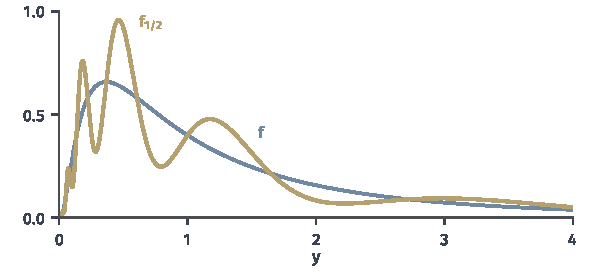
\includegraphics[width=100mm]{figures/07-probability/03-probability-limits/matplotlib/weak-lognormal/figure.pdf}
 \caption{各阶矩相同的两个密度。蓝线为对数正态密度$f$，黄线为$f_{1/2}(y)=f(y)(1+\frac12\sin(2\pi\ln y))$。脚本用数值积分核对了二者的前四阶矩都等于$\mathrm{e}^{k^2/2}$。}
 \label{fig:weak-lognormal}
\end{BookInlineFigure}

\paragraph{两种表示的分工}
下表比较两种变换。特征函数总存在，识别分布与刻画弱收敛都不需要附加条件；矩母函数是实值的，便于计算矩和尾部的指数界，但只有在$0$的邻域上有限时才能用于识别。下一章证明中心极限定理时只假定方差有限，矩母函数可能处处无穷（例如$t$分布），所以证明用特征函数，不以矩母函数存在作为前提。

\begin{BookInlineTable}
 \centering
 \caption{特征函数与矩母函数}
 \label{tab:weak-cf-mgf}
 \begin{tabular}{@{}lll@{}}
 \toprule
 & 特征函数$\phi_X(t)$ & 矩母函数$M_X(t)$\\
 \midrule
 存在范围 & 一切$t$，模不超过$1$ & 区间$D_X$，可能只有$\{0\}$\\
 读出矩 & $k$阶矩有限时求$k$次导 & $0$的邻域有限时全部矩\\
 识别分布 & 无条件 & 需$0$的邻域有限\\
 收敛判据 & 连续性定理 & 需$0$的邻域上收敛\\
 独立和 & 乘积 & 乘积（在有限处）\\
 \bottomrule
 \end{tabular}
\end{BookInlineTable}


\section{连续映射}
\label{sec:weak-continuous-mapping}

已知$X_n\xrightarrow{\mathrm{d}}X$，常常还要知道$X_n^{2}$、$\mathrm{e}^{X_n}$、$\mathbf{1}_{\{X_n>a\}}$或$1/X_n$的极限。对每个$X_n$作同一个确定的变换$g$，极限能否随之传递？若$g$连续，答案几乎写在定义里：对$f\in C_b$，复合$f\circ g$仍是有界连续函数，所以
\[
 \mathbb{E}\bigl[f(g(\bm{X}_n))\bigr]=\mathbb{E}\bigl[(f\circ g)(\bm{X}_n)\bigr]\longrightarrow\mathbb{E}\bigl[(f\circ g)(\bm{X})\bigr]=\mathbb{E}\bigl[f(g(\bm{X}))\bigr] .
\]

实际要用的$g$常有不连续点：阈值的示性函数在阈值处跳跃，倒数在$0$处没有定义。下面的定理允许$g$有不连续点，只要极限分布不把质量放在那里。

\begin{theorem}[连续映射定理]
\label{thm:weak-continuous-mapping}
设$\bm{X}_n\xrightarrow{\mathrm{d}}\bm{X}$，$\bm{X}_n,\bm{X}$取值于$\mathbb{R}^{d}$。设$g:\mathbb{R}^{d}\to\mathbb{R}^{k}$为Borel可测映射，$D_g$为它的不连续点集。若$\mathbb{P}(\bm{X}\in D_g)=0$，则$g(\bm{X}_n)\xrightarrow{\mathrm{d}}g(\bm{X})$。
\end{theorem}

\begin{proof}
可以证明$D_g$是Borel集，所以$\mathbb{P}(\bm{X}\in D_g)$有意义。用Portmanteau定理的(3)验证。取$\mathbb{R}^{k}$中的闭集$F$，记$\overline{g^{-1}(F)}$为原像的闭包。

先说明$\overline{g^{-1}(F)}\subset g^{-1}(F)\cup D_g$。设$\bm{x}$在闭包中，取$\bm{x}_m\in g^{-1}(F)$，$\bm{x}_m\to\bm{x}$。若$g$在$\bm{x}$处连续，则$g(\bm{x})=\lim g(\bm{x}_m)$，而$g(\bm{x}_m)\in F$，$F$闭，所以$g(\bm{x})\in F$，即$\bm{x}\in g^{-1}(F)$。否则$\bm{x}\in D_g$。

于是，由原像的闭包是闭集，以及$\bm{X}_n\xrightarrow{\mathrm{d}}\bm{X}$与Portmanteau定理的(3)，
\[
 \begin{aligned}
 \limsup_{n\to\infty}\mathbb{P}\bigl(g(\bm{X}_n)\in F\bigr)
 &\leq\limsup_{n\to\infty}\mathbb{P}\bigl(\bm{X}_n\in\overline{g^{-1}(F)}\bigr)
 \leq\mathbb{P}\bigl(\bm{X}\in\overline{g^{-1}(F)}\bigr)\\
 &\leq\mathbb{P}\bigl(\bm{X}\in g^{-1}(F)\bigr)+\mathbb{P}(\bm{X}\in D_g)=\mathbb{P}\bigl(g(\bm{X})\in F\bigr) .
 \end{aligned}
\]
再用一次Portmanteau定理即得结论。
\end{proof}

定理~\ref{thm:weak-continuous-mapping}通称\term{连续映射定理}（continuous mapping theorem）。条件$\mathbb{P}(\bm{X}\in D_g)=0$只涉及极限$\bm{X}$，与$\bm{X}_n$是否把质量放在$D_g$上无关。这与Portmanteau定理(5)的边界条件是同一种要求：示性函数$\mathbf{1}_A$的不连续点集正是$\partial A$。

\paragraph{阈值}
设$g(x)=\mathbf{1}_{\{x>1/2\}}$，$D_g=\{1/2\}$。对格点均匀分布，$U_n\xrightarrow{\mathrm{d}}U\sim\operatorname{Unif}(0,1)$，且$\mathbb{P}(U=1/2)=0$，所以$\mathbf{1}_{\{U_n>1/2\}}\xrightarrow{\mathrm{d}}\operatorname{Bern}(1/2)$。直接计算也是如此：$\mathbb{P}(U_n>1/2)=1-\lfloor n/2\rfloor/n\to1/2$。

换成$\delta_{1/n}\to\delta_0$与阈值$0$，$g(x)=\mathbf{1}_{\{x>0\}}$，则$g(1/n)=1$恒成立，而$g(0)=0$。极限分布的全部质量都在$D_g=\{0\}$上，条件不满足，结论确实失败。图~\ref{fig:weak-threshold-mapping}并列了这两种情形。

\begin{BookInlineFigure}
 \centering
 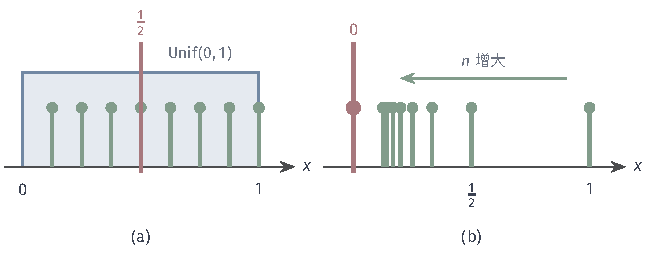
\includegraphics[width=110.6mm]{figures/07-probability/03-probability-limits/tikz/weak-threshold-mapping/figure.pdf}
 \caption{阈值映射与极限质量的位置。(a)格点均匀分布$U_8$的质点（绿）与极限$\operatorname{Unif}(0,1)$的密度（浅蓝），阈值$1/2$（红色竖线）处$U_8$有质量而极限没有，阈值右侧的概率收敛到$1/2$。(b)$\delta_{1/n}$的质点（绿）从右侧逼近阈值$0$，极限$\delta_0$（红点）恰好落在阈值上，$\mathbf{1}_{\{X_n>0\}}$恒为$1$，极限却是$0$。}
 \label{fig:weak-threshold-mapping}
\end{BookInlineFigure}

\paragraph{倒数}
令$g(x)=1/x$（$x\neq0$），$g(0)=0$，则$D_g=\{0\}$。若$X_n\xrightarrow{\mathrm{d}}X$且$\mathbb{P}(X=0)=0$，则$1/X_n\xrightarrow{\mathrm{d}}1/X$。$g(0)$取什么值无关紧要，它只影响$X_n=0$的样本，而极限分布不关心那里。

仍以格点均匀分布为例，$\mathbb{P}(U=0)=0$，所以$1/U_n\xrightarrow{\mathrm{d}}1/U$。极限的右尾为
\[
 \mathbb{P}(1/U>y)=\mathbb{P}(U<1/y)=\frac1y,\qquad y\geq1 ,
\]
这是第~\ref{chap:tail-probabilities}章参数为$1$的Pareto分布，没有期望。直接计算，$U_n<1/y$的格点是$k<n/y$，个数为$\lceil n/y\rceil-1$，于是
\[
 \mathbb{P}(1/U_n>y)=\frac{\lceil n/y\rceil-1}{n}\longrightarrow\frac1y .
\]
注意每个$1/U_n$都不超过$n$，有界；极限却是重尾分布。图~\ref{fig:weak-reciprocal}(a)画出这一收敛。

分母趋于零时条件就会失效。设$X_n=(-1)^{n}/n$，则$X_n\xrightarrow{\mathrm{d}}0$，极限把全部质量放在$D_g$上。$1/X_n=(-1)^{n}n$在$\pm\infty$之间来回跳，没有任何弱极限。即使取$X_n\sim\mathcal{N}(0,1/n^{2})$这样处处没有原子的分布，$1/X_n$的分布也是$1/X_1$的分布按$n$倍放大，质量逃向无穷远，见图~\ref{fig:weak-reciprocal}(b)。

\begin{BookInlineFigure}
 \centering
 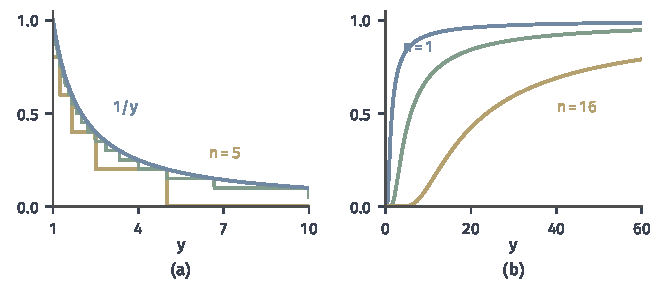
\includegraphics[width=112mm]{figures/07-probability/03-probability-limits/matplotlib/weak-reciprocal/figure.pdf}
 \caption{倒数映射。(a)$\mathbb{P}(1/U_n>y)$，$n=5$（黄）与$n=20$（绿），蓝线为极限$1/y$。(b)$X_n\sim\mathcal{N}(0,1/n^2)$时$\lvert1/X_n\rvert$的分布函数，$n=1$（蓝）、$4$（绿）、$16$（黄），曲线整体右移，质量逃向无穷远。}
 \label{fig:weak-reciprocal}
\end{BookInlineFigure}

连续映射定理处理的是同一个确定变换。若变换本身也随$n$变化，例如$g_n(x)=x+1/n$，则要另外论证；若变换涉及两个随机变量，例如$X_n+Y_n$，则需要$(X_n,Y_n)$作为一个随机向量的极限，这是下一节的问题。


\section{联合收敛}
\label{sec:weak-joint}

设$X_n\xrightarrow{\mathrm{d}}X$，$Y_n\xrightarrow{\mathrm{d}}Y$。$X_n+Y_n$的极限是什么？这个问题在只知道两个边缘极限时没有答案，因为$X+Y$的分布取决于$X$与$Y$怎样配对，而边缘分布不含配对的信息。本节先把联合收敛与边缘收敛分开，再给出两类常用的判据：方向投影，以及一个分量趋于常量的情形。有了联合极限，上一节的连续映射定理就可以处理和、积与比。

\subsection{边缘收敛与联合收敛}
\label{sec:weak-marginal-joint}

设$(\bm{X}_n,\bm{Y}_n)$是取值于$\mathbb{R}^{d}\times\mathbb{R}^{k}$的随机向量，即每个$n$下$\bm{X}_n$与$\bm{Y}_n$定义在同一个概率空间上。联合收敛$(\bm{X}_n,\bm{Y}_n)\xrightarrow{\mathrm{d}}(\bm{X},\bm{Y})$就是这个$(d+k)$维随机向量的依分布收敛。坐标投影$(\bm{x},\bm{y})\mapsto\bm{x}$连续，由连续映射定理，联合收敛推出$\bm{X}_n\xrightarrow{\mathrm{d}}\bm{X}$与$\bm{Y}_n\xrightarrow{\mathrm{d}}\bm{Y}$。

反过来不成立。设$Z\sim\mathcal{N}(0,1)$，令
\[
 X_n=Z,\qquad Y_n=(-1)^{n}Z .
\]
$-Z$也服从$\mathcal{N}(0,1)$，所以两个边缘分布对每个$n$都是$\mathcal{N}(0,1)$，边缘平凡地收敛。联合分布却在两种之间交替：偶数$n$时$(Z,Z)$落在直线$y=x$上，奇数$n$时$(Z,-Z)$落在$y=-x$上。取有界连续函数$f(x,y)=\min(1,\lvert x-y\rvert)$，偶数项的读数为$0$，奇数项为$\mathbb{E}[\min(1,2\lvert Z\rvert)]>0$，所以联合分布没有极限。图~\ref{fig:weak-pairings}画出这两种配对，以及同样边缘下的第三种配对：独立。

\begin{BookInlineFigure}
 \centering
 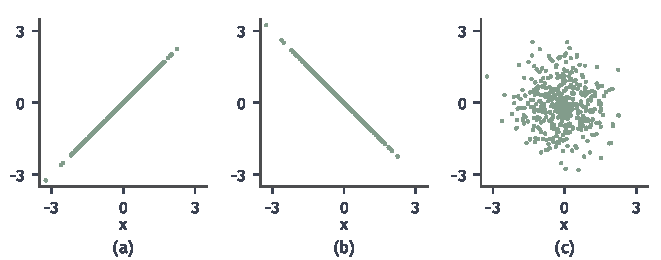
\includegraphics[width=112mm]{figures/07-probability/03-probability-limits/matplotlib/weak-pairings/figure.pdf}
 \caption{边缘相同、配对不同。三幅图各有$400$个样本点（种子$7$），两个坐标的边缘分布都是$\mathcal{N}(0,1)$。(a)$(Z,Z)$；(b)$(Z,-Z)$；(c)$(Z,Z')$，$Z'$与$Z$独立同分布。}
 \label{fig:weak-pairings}
\end{BookInlineFigure}

\paragraph{各分量独立的情形}
若对每个$n$，$\bm{X}_n$与$\bm{Y}_n$独立，配对方式就被固定下来，边缘收敛足以推出联合收敛。

\begin{theorem}[独立分量的联合极限]
\label{thm:weak-independent-joint}
设对每个$n$，$\bm{X}_n$与$\bm{Y}_n$定义在同一概率空间上且相互独立，$\bm{X}_n\xrightarrow{\mathrm{d}}\bm{X}$，$\bm{Y}_n\xrightarrow{\mathrm{d}}\bm{Y}$。则$(\bm{X}_n,\bm{Y}_n)\xrightarrow{\mathrm{d}}(\bm{X},\bm{Y})$，其中$\bm{X}$与$\bm{Y}$独立，即极限分布是$P_{\bm{X}}$与$P_{\bm{Y}}$的乘积。
\end{theorem}

\begin{proof}
由式~\eqref{eq:weak-cf-joint-independent}与连续性定理的(1)，
\[
 \phi_{(\bm{X}_n,\bm{Y}_n)}(\bm{s},\bm{t})=\phi_{\bm{X}_n}(\bm{s})\,\phi_{\bm{Y}_n}(\bm{t})\longrightarrow\phi_{\bm{X}}(\bm{s})\,\phi_{\bm{Y}}(\bm{t}) .
\]
取$\bm{X}$与$\bm{Y}$独立，右边正是$(\bm{X},\bm{Y})$的特征函数，它连续。由连续性定理的(2)，结论成立。
\end{proof}

定理只要求同一个$n$下的两个分量独立，不要求不同$n$之间有任何关系；各个$n$甚至可以在不同的概率空间上。例如每个$n$下独立地取$X_n\sim\operatorname{Bin}(n,2/n)$与格点均匀分布$U_n$，则$(X_n,U_n)$依分布收敛到$\operatorname{Poisson}(2)$与$\operatorname{Unif}(0,1)$的乘积分布。

\subsection{Cramér--Wold判据}
\label{sec:weak-cramer-wold}

一般的联合分布怎样检验？直接用多元特征函数可以，但常常更方便的是把向量投影到一个方向上，化为一维问题。投影$\langle\bm{a},\bm{X}\rangle$的特征函数在$1$处的值是
\[
 \phi_{\langle\bm{a},\bm{X}\rangle}(1)=\mathbb{E}\bigl[\mathrm{e}^{\mathrm{i}\langle\bm{a},\bm{X}\rangle}\bigr]=\phi_{\bm{X}}(\bm{a}) .
\]
所以多元特征函数在$\bm{a}$处的值，就是沿方向$\bm{a}$的一维投影的信息。知道所有方向的投影分布，就知道整个多元特征函数。

\begin{theorem}[Cramér--Wold判据]
\label{thm:weak-cramer-wold}
设$\bm{X}_n,\bm{X}$取值于$\mathbb{R}^{d}$。则$\bm{X}_n\xrightarrow{\mathrm{d}}\bm{X}$，当且仅当对每个$\bm{a}\in\mathbb{R}^{d}$，
\begin{equation}
 \langle\bm{a},\bm{X}_n\rangle\xrightarrow{\mathrm{d}}\langle\bm{a},\bm{X}\rangle .
 \label{eq:weak-cramer-wold}
\end{equation}
特别地，$\bm{X}$的分布由全部一维投影$\langle\bm{a},\bm{X}\rangle$的分布确定。
\end{theorem}

\begin{proof}
必要性：$\bm{x}\mapsto\langle\bm{a},\bm{x}\rangle$连续，由连续映射定理。充分性：由式~\eqref{eq:weak-cramer-wold}与连续性定理的(1)，对每个$\bm{a}$，
\[
 \phi_{\bm{X}_n}(\bm{a})=\phi_{\langle\bm{a},\bm{X}_n\rangle}(1)\longrightarrow\phi_{\langle\bm{a},\bm{X}\rangle}(1)=\phi_{\bm{X}}(\bm{a}) .
\]
极限$\phi_{\bm{X}}$连续，由连续性定理的(2)得$\bm{X}_n\xrightarrow{\mathrm{d}}\bm{X}$。最后一句：若$\bm{X}$与$\bm{Y}$的各个投影同分布，则$\phi_{\bm{X}}(\bm{a})=\phi_{\bm{Y}}(\bm{a})$对一切$\bm{a}$成立，由定理~\ref{thm:weak-cf-uniqueness}得$P_{\bm{X}}=P_{\bm{Y}}$。
\end{proof}

这个判据也称为\term{Cramér--Wold方法}（Cramér--Wold device）。判据要求所有方向，坐标方向只是$\bm{a}=\bm{e}_j$这$d$个特例，它们只给出边缘分布。上一小节的例子已经说明边缘不够；下面看一个固定的随机向量，它的坐标方向都是高斯，某个斜方向却不是。

\paragraph{联合高斯的判别}
第~\ref{chap:multivariate-distributions}章说过：若每个线性组合$\langle\bm{a},\bm{X}\rangle$都服从一元高斯分布（方差可以为$0$），则$\bm{X}$联合高斯。现在可以证明。每个坐标服从高斯分布，所以二阶矩有限，记$\bm{\mu}=\mathbb{E}[\bm{X}]$，$\bm{\Sigma}$为协方差矩阵。$\langle\bm{a},\bm{X}\rangle$的均值为$\langle\bm{a},\bm{\mu}\rangle$，方差为$\bm{a}^{\top}\bm{\Sigma}\bm{a}$，按假设它是高斯的，于是
\[
 \phi_{\bm{X}}(\bm{a})=\phi_{\langle\bm{a},\bm{X}\rangle}(1)=\exp\Bigl(\mathrm{i}\langle\bm{a},\bm{\mu}\rangle-\frac12\bm{a}^{\top}\bm{\Sigma}\bm{a}\Bigr) .
\]
这正是式~\eqref{eq:weak-mvn-cf}中$\mathcal{N}(\bm{\mu},\bm{\Sigma})$的特征函数，由定理~\ref{thm:weak-cf-uniqueness}，$\bm{X}\sim\mathcal{N}(\bm{\mu},\bm{\Sigma})$。

那一章还给出了只检查坐标方向不够的例子。$Z\sim\mathcal{N}(0,1)$，$S$以各$1/2$的概率取$\pm1$且与$Z$独立，$\bm{X}=(Z,SZ)$。两个坐标都服从$\mathcal{N}(0,1)$，由独立性，协方差$\mathbb{E}[SZ^{2}]$等于$\mathbb{E}[S]\,\mathbb{E}[Z^{2}]=0$。若$\bm{X}$联合高斯，它就是$\mathcal{N}(\bm{0},\bm{I}_2)$，方向$\bm{a}=(1,1)$上的投影应服从$\mathcal{N}(0,2)$。实际上
\[
 Z+SZ=(1+S)Z=\begin{cases}2Z,&S=1,\\0,&S=-1,\end{cases}
\]
它以概率$1/2$恰好等于$0$，不是高斯分布。图~\ref{fig:weak-cramer-wold}(a)是$\bm{X}$的样本，全部落在两条对角线上；(b)是这个斜方向投影的分布。

\begin{BookInlineFigure}
 \centering
 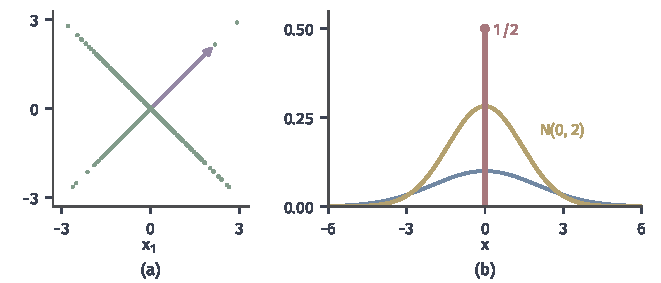
\includegraphics[width=112mm]{figures/07-probability/03-probability-limits/matplotlib/weak-cramer-wold/figure.pdf}
 \caption{坐标方向都是高斯，斜方向不是。(a)$\bm{X}=(Z,SZ)$的$600$个样本（种子$11$），两个边缘都是$\mathcal{N}(0,1)$，紫色箭头为方向$(1,1)$。(b)$Z+SZ$的分布：$0$处质量$1/2$的原子（红色竖线），其余质量的密度为$\frac12$乘$\mathcal{N}(0,4)$的密度（蓝）；黄线为假如联合高斯时应有的$\mathcal{N}(0,2)$密度。}
 \label{fig:weak-cramer-wold}
\end{BookInlineFigure}

Cramér--Wold判据适用于固定的有限维数$d$。下一章的多元中心极限定理正是用它把各个方向上的一维极限合成联合高斯极限。

\subsection{Slutsky定理}
\label{sec:weak-slutsky}

联合收敛有一个特别好用的情形：一个分量依分布收敛，另一个依概率趋于常量。常量没有随机性，不存在配对问题，所以边缘信息就够了。典型的场合是用一个依概率收敛的量替换未知的常数，例如第~\ref{chap:laws-of-large-numbers}章的大数律给出的样本平均。

\begin{theorem}[Slutsky定理]
\label{thm:weak-slutsky}
设对每个$n$，$\bm{X}_n$与$\bm{Y}_n$定义在同一概率空间上，分别取值于$\mathbb{R}^{d}$与$\mathbb{R}^{k}$。若$\bm{X}_n\xrightarrow{\mathrm{d}}\bm{X}$，且对常向量$\bm{c}\in\mathbb{R}^{k}$有$\bm{Y}_n\xrightarrow{\mathbb{P}}\bm{c}$，则
\begin{equation}
 (\bm{X}_n,\bm{Y}_n)\xrightarrow{\mathrm{d}}(\bm{X},\bm{c}) .
 \label{eq:weak-slutsky-joint}
\end{equation}
因此，对实随机变量$X_n\xrightarrow{\mathrm{d}}X$与$Y_n\xrightarrow{\mathbb{P}}c$，
\begin{equation}
 X_n+Y_n\xrightarrow{\mathrm{d}}X+c,\qquad Y_nX_n\xrightarrow{\mathrm{d}}cX,\qquad X_n/Y_n\xrightarrow{\mathrm{d}}X/c\quad(c\neq0) .
 \label{eq:weak-slutsky}
\end{equation}
\end{theorem}

\begin{proof}
由Portmanteau定理的(2)，只需对有界Lipschitz函数$f$验证。设$\lvert f\rvert\leq M$，Lipschitz常数为$L$。任取$\varepsilon>0$，把差拆成两部分：
\[
 \begin{aligned}
 \bigl\lvert\mathbb{E}[f(\bm{X}_n,\bm{Y}_n)]-\mathbb{E}[f(\bm{X},\bm{c})]\bigr\rvert
 &\leq\mathbb{E}\bigl[\lvert f(\bm{X}_n,\bm{Y}_n)-f(\bm{X}_n,\bm{c})\rvert\bigr]\\
 &\quad+\bigl\lvert\mathbb{E}[f(\bm{X}_n,\bm{c})]-\mathbb{E}[f(\bm{X},\bm{c})]\bigr\rvert .
 \end{aligned}
\]

第一部分在$\lVert\bm{Y}_n-\bm{c}\rVert_2<\varepsilon$时被$L\varepsilon$控制，其余情形被$2M$控制，所以不超过
\[
 L\varepsilon+2M\,\mathbb{P}\bigl(\lVert\bm{Y}_n-\bm{c}\rVert_2\geq\varepsilon\bigr) ,
\]
后一项趋于零。第二部分中，$\bm{x}\mapsto f(\bm{x},\bm{c})$有界连续，由$\bm{X}_n\xrightarrow{\mathrm{d}}\bm{X}$趋于零。于是左边的上极限不超过$L\varepsilon$，$\varepsilon$任意，式~\eqref{eq:weak-slutsky-joint}成立。

式~\eqref{eq:weak-slutsky}中，$(x,y)\mapsto x+y$与$(x,y)\mapsto xy$连续。$(x,y)\mapsto x/y$只在直线$y=0$上不连续，而$(X,c)$落在这条直线上的概率在$c\neq0$时为零。由连续映射定理即得。
\end{proof}

\term{Slutsky定理}（Slutsky's theorem）不要求$\bm{X}_n$与$\bm{Y}_n$独立，它们可以有任意的依赖关系；证明的第一部分只用了$\bm{Y}_n$靠近$\bm{c}$的概率，没有用到$\bm{Y}_n$与$\bm{X}_n$怎样配对。这里只需要每个$n$下二者在同一空间上，使$(\bm{X}_n,\bm{Y}_n)$有意义。

看一个强依赖的例子。设$X\sim\mathcal{N}(0,1)$，令$X_n=X$，$Y_n=1+X/\sqrt{n}$。则$Y_n-1=X/\sqrt n\to0$对每个样本点成立，$Y_n\xrightarrow{\mathbb{P}}1$，而$Y_n$完全由$X_n$决定。$\mathbb{P}(Y_n=0)=0$，比值有定义，由Slutsky定理，
\[
 \frac{X_n}{Y_n}=\frac{X}{1+X/\sqrt{n}}\xrightarrow{\mathrm{d}}\mathcal{N}(0,1) .
\]
有限的$n$下，分母可能很接近$0$，比值有很重的尾部；$n$增大，这种情形的概率越来越小。图~\ref{fig:weak-slutsky}用模拟显示了这个过程。

\begin{BookInlineFigure}
 \centering
 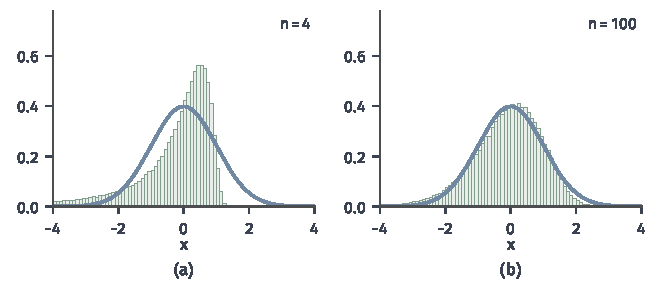
\includegraphics[width=112mm]{figures/07-probability/03-probability-limits/matplotlib/weak-slutsky/figure.pdf}
 \caption{Slutsky定理中的依赖分母。$X\sim\mathcal{N}(0,1)$，$X/(1+X/\sqrt n)$的直方图（浅绿，$2\times10^{5}$个样本，种子$3$，只画$[-4,4]$内的部分），蓝线为$\mathcal{N}(0,1)$的密度。(a)$n=4$，左侧的长尾来自分母接近零的样本；(b)$n=100$。}
 \label{fig:weak-slutsky}
\end{BookInlineFigure}

\paragraph{条件的作用}
常量分母必须非零。$X_n=Z\sim\mathcal{N}(0,1)$，$Y_n=1/n\xrightarrow{\mathbb{P}}0$，则$X_n/Y_n=nZ\sim\mathcal{N}(0,n^{2})$，质量逃向无穷远，没有弱极限。

常量也不能换成一般的随机极限。设$X_n=Z$，$Y_n=(-1)^{n}Z$，则$X_n\xrightarrow{\mathrm{d}}Z$，$Y_n\xrightarrow{\mathrm{d}}Z$，但
\[
 X_n+Y_n=\begin{cases}2Z,&n\text{为偶数},\\0,&n\text{为奇数}\end{cases}
\]
没有极限。两个分量各自依分布收敛到非退化的分布时，必须另外知道它们的联合收敛，例如由定理~\ref{thm:weak-independent-joint}的独立条件或由Cramér--Wold判据得到，才能谈论和的极限。


\section{分布积分的极限}
\label{sec:weak-integral-limits}

弱收敛控制的是有界连续函数的期望。可是最常用的量，均值、方差、高阶矩，都是无界函数的期望。设$X_n\xrightarrow{\mathrm{d}}X$，$g$连续而无界，$\mathbb{E}[g(X_n)]$是否趋于$\mathbb{E}[g(X)]$？

第~\ref{sec:weak-mass-control}节的例子给出否定的回答。$X_n$以概率$1/n$取$n$、否则取$0$。对$f\in C_b$，$\mathbb{E}[f(X_n)]=(1-1/n)f(0)+f(n)/n\to f(0)$，所以$X_n\xrightarrow{\mathrm{d}}0$。可是
\[
 \mathbb{E}[X_n]=n\cdot\frac1n=1\quad\text{对一切}n,\qquad\mathbb{E}[0]=0 .
\]
远处那份越来越轻的质量，乘以越来越大的位置，始终贡献$1$。弱收敛看不到它，因为有界函数在远处的读数被$\sup\lvert f\rvert/n$压住了；期望却要乘以位置本身。每个$X_n$的各阶矩都有限，$\mathbb{E}[X_n^{k}]=n^{k-1}$，但这对极限毫无帮助。

\paragraph{一致可积条件}
补上的条件正是第~\ref{sec:weak-mass-control}节对比过的一致可积：要求远处质量乘以位置之后，对所有$n$一致地小。

\begin{theorem}[期望的收敛]
\label{thm:weak-ui-expectation}
设$\bm{X}_n\xrightarrow{\mathrm{d}}\bm{X}$，$g:\mathbb{R}^{d}\to\mathbb{R}$可测，$\mathbb{P}(\bm{X}\in D_g)=0$，并且$\{g(\bm{X}_n)\}$一致可积：
\begin{equation}
 \lim_{r\to\infty}\sup_{n}\mathbb{E}\bigl[\lvert g(\bm{X}_n)\rvert\,\mathbf{1}_{\{\lvert g(\bm{X}_n)\rvert>r\}}\bigr]=0 .
 \label{eq:weak-ui}
\end{equation}
则$\mathbb{E}[\lvert g(\bm{X})\rvert]<\infty$，并且
\begin{equation}
 \lim_{n\to\infty}\mathbb{E}\bigl[g(\bm{X}_n)\bigr]=\mathbb{E}\bigl[g(\bm{X})\bigr] .
 \label{eq:weak-ui-expectation}
\end{equation}
\end{theorem}

\begin{proof}
记$Y_n=g(\bm{X}_n)$，$Y=g(\bm{X})$。由连续映射定理，$Y_n\xrightarrow{\mathrm{d}}Y$，于是问题化为实随机变量。对$r>0$，令截断函数
\[
 h_r(y)=\max\bigl(-r,\min(y,r)\bigr) ,
\]
它有界连续，与$y$只在$\lvert y\rvert>r$处不同，并且在那里与$y$之差的绝对值不超过$\lvert y\rvert$。

先证$Y$可积。$y\mapsto\min(\lvert y\rvert,r)$有界连续，所以
\[
 \mathbb{E}\bigl[\min(\lvert Y\rvert,r)\bigr]=\lim_{n\to\infty}\mathbb{E}\bigl[\min(\lvert Y_n\rvert,r)\bigr]\leq\sup_{n}\mathbb{E}\bigl[\lvert Y_n\rvert\bigr] .
\]
由式~\eqref{eq:weak-ui}，取$r_0$使尾部积分不超过$1$，则$\mathbb{E}[\lvert Y_n\rvert]\leq r_0+1$，右边有限。令$r\to\infty$，由单调收敛定理，$\mathbb{E}[\lvert Y\rvert]\leq r_0+1<\infty$。

再拆三项。对每个$r$，
\[
 \begin{aligned}
 \bigl\lvert\mathbb{E}[Y_n]-\mathbb{E}[Y]\bigr\rvert
 &\leq\mathbb{E}\bigl[\lvert Y_n\rvert\mathbf{1}_{\{\lvert Y_n\rvert>r\}}\bigr]+\bigl\lvert\mathbb{E}[h_r(Y_n)]-\mathbb{E}[h_r(Y)]\bigr\rvert\\
 &\quad+\mathbb{E}\bigl[\lvert Y\rvert\mathbf{1}_{\{\lvert Y\rvert>r\}}\bigr] .
 \end{aligned}
\]
任取$\varepsilon>0$。由式~\eqref{eq:weak-ui}，取$r$使第一项对一切$n$不超过$\varepsilon$；$Y$可积，由支配收敛定理，$r$足够大时第三项也不超过$\varepsilon$。固定这个$r$，令$n\to\infty$，第二项趋于零。于是左边的上极限不超过$2\varepsilon$。
\end{proof}

证明中“先证可积”这一步本身给出一个不需要一致可积的结论：只要$Y_n\xrightarrow{\mathrm{d}}Y$，就有
\begin{equation}
 \mathbb{E}\bigl[\lvert Y\rvert\bigr]\leq\liminf_{n\to\infty}\mathbb{E}\bigl[\lvert Y_n\rvert\bigr] .
 \label{eq:weak-fatou}
\end{equation}
推导时把$\sup_n$换成$\liminf_n$即可。它是Fatou引理在依分布收敛下的形式：极限只可能丢失期望，不会凭空增加。开头的例子中，$\mathbb{E}[X_n]=1$，极限的期望$0$严格变小，丢失的正是逃到远处的那一份。

一致可积常用矩条件验证。若存在$\delta>0$与常数$C$，使$\mathbb{E}[\lvert Y_n\rvert^{1+\delta}]\leq C$对一切$n$成立，则由于在$\lvert y\rvert>r$处$(\lvert y\rvert/r)^{\delta}>1$，
\[
 \sup_n\mathbb{E}\bigl[\lvert Y_n\rvert\mathbf{1}_{\{\lvert Y_n\rvert>r\}}\bigr]\leq\frac{C}{r^{\delta}}\longrightarrow0 .
\]
注意要的是比一阶稍高的矩的一致界；开头的例子中，每个$X_n$的高阶矩虽然有限，却没有一致界。

\paragraph{二项分布的矩}
$X_n\sim\operatorname{Bin}(n,2/n)\xrightarrow{\mathrm{d}}N\sim\operatorname{Poisson}(2)$。二阶矩是否收敛？可以直接计算：
\[
 \mathbb{E}[X_n^{2}]=\operatorname{Var}(X_n)+(\mathbb{E}[X_n])^{2}=2\Bigl(1-\frac2n\Bigr)+4=6-\frac4n\longrightarrow6=\mathbb{E}[N^{2}] .
\]
用定理~\ref{thm:weak-ui-expectation}也能得到，并且不需要精确的公式，只要一个三阶矩的界。

$X_n(X_n-1)(X_n-2)$等于从成功的试验中按顺序取出三个不同试验的方式数，每个有序三元组全部成功的概率为$p^{3}$，这里$p=2/n$，所以
\[
 \mathbb{E}[X_n(X_n-1)(X_n-2)]=n(n-1)(n-2)p^{3}\leq(np)^{3}=8 .
\]
同理$\mathbb{E}[X_n(X_n-1)]\leq(np)^{2}=4$。由$x^{3}=x(x-1)(x-2)+3x(x-1)+x$，
\[
 \mathbb{E}[X_n^{3}]\leq8+3\cdot4+2=22 .
\]
取$Y_n=X_n^{2}$，$\delta=1/2$，$\sup_n\mathbb{E}[\lvert Y_n\rvert^{3/2}]\leq22$，所以$\{X_n^{2}\}$一致可积，$\mathbb{E}[X_n^{2}]\to\mathbb{E}[N^{2}]$。同样的论证对任意阶矩都适用。图~\ref{fig:weak-ui-truncation}把这个例子与开头的反例并列。

\begin{BookInlineFigure}
 \centering
 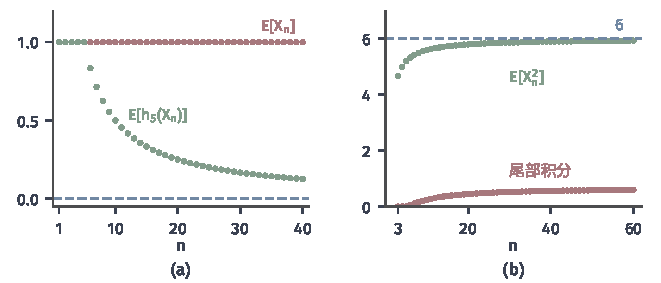
\includegraphics[width=112mm]{figures/07-probability/03-probability-limits/matplotlib/weak-ui-truncation/figure.pdf}
 \caption{期望能否随分布取极限。(a)$X_n$以概率$1/n$取$n$：$\mathbb{E}[X_n]$（红）恒为$1$，截断期望$\mathbb{E}[h_5(X_n)]$（绿）趋于极限的期望$0$（蓝色虚线），二者之差是$r=5$以外的尾部积分。(b)$X_n\sim\operatorname{Bin}(n,2/n)$：$\mathbb{E}[X_n^2]$（绿）趋于$6$（蓝色虚线），尾部积分$\mathbb{E}[X_n^2\mathbf{1}_{\{X_n^2>25\}}]$（红）对一切$n$都小于$0.7$，不随$n$增长。}
 \label{fig:weak-ui-truncation}
\end{BookInlineFigure}

\paragraph{与\texorpdfstring{$L^{1}$}{L1}收敛判据的区别}
第~\ref{chap:random-variable-convergence}章在同一概率空间上证明过：$X_n\xrightarrow{\mathbb{P}}X$且$\{X_n\}$一致可积，当且仅当$X_n\xrightarrow{L^{1}}X$，即$\mathbb{E}[\lvert X_n-X\rvert]\to0$。定理~\ref{thm:weak-ui-expectation}用的也是一致可积，但结论弱得多：它只说期望这一个数收敛，不涉及$\lvert X_n-X\rvert$，这个差可能根本没有定义。第~\ref{sec:weak-test-functions}节中$X(\omega)=\omega$、$X_n(\omega)=1-\omega$的例子里，期望恒等，而$\lvert1-2\omega\rvert$的平均$\mathbb{E}[\lvert X_n-X\rvert]=1/2$不趋于零。

\paragraph{不是期望的量}
定理处理的是固定函数$g$的期望。有些量由整个质量表或密度计算，不能写成某个固定$g$的期望，例如第~\ref{chap:information-measures}章的熵；弱收敛对它们没有一般的保证。格点均匀分布就是一例：$U_n$的质量表是$n$个$1/n$，任何只依赖各点质量大小的量都与$\operatorname{Unif}(0,1)$的密度无从比较，尽管$U_n\xrightarrow{\mathrm{d}}\operatorname{Unif}(0,1)$。这类量的极限要在相应的章节里另加条件讨论。


\section{本章小结}
\label{sec:weak-summary}

章首的两个例子，$\operatorname{Bin}(n,2/n)$趋于$\operatorname{Poisson}(2)$与格点均匀分布趋于$\operatorname{Unif}(0,1)$，现在都有了确切的含义：对每个有界连续函数，分布下的平均收敛。这个定义只比较分布，不要求随机变量在同一空间上，也不断言样本彼此接近；在共同空间上，依概率收敛推出依分布收敛，反之只在极限为常量时成立。有界保证读数存在，连续让质点位置的微小移动只引起读数的微小变化。

本章的工具按承担的任务可以分成几类，各有各的条件，见表~\ref{tab:weak-summary}。

\begin{BookInlineTable}
 \centering
 \caption{弱收敛的工具及其条件}
 \label{tab:weak-summary}
 \begin{tabular}{@{}lll@{}}
 \toprule
 任务 & 工具 & 关键条件\\
 \midrule
 事件概率 & Portmanteau定理 & 极限在事件边界上无质量\\
 实轴上的判据 & 分布函数判据 & 只在极限分布函数的连续点\\
 极限的存在 & 胎紧与弱收敛子列 & 远处质量一致地小\\
 极限的识别 & 特征函数唯一性 & 无\\
 收敛的判别 & 连续性定理 & 逐点极限在原点连续\\
 另一种表示 & 矩母函数 & 在$0$的邻域上有限\\
 映射的传递 & 连续映射定理 & 极限不在不连续点集上\\
 联合极限 & Cramér--Wold判据 & 检查所有方向的投影\\
 常量替换 & Slutsky定理 & 一个分量依概率趋于常量\\
 期望的极限 & 一致可积 & 远处质量乘位置一致地小\\
 \bottomrule
 \end{tabular}
\end{BookInlineTable}

几组容易混淆的区别值得再强调。胎紧控制远处有多少质量，一致可积还要乘上位置：前者决定极限分布是否存在，后者决定期望是否随之收敛。特征函数总存在，识别分布不需要任何条件；矩母函数只在零点邻域有限时才能识别，对数正态分布说明所有矩有限也不够。边缘收敛不推出联合收敛，坐标方向的投影也不能代替所有方向；只有一个分量的极限是常量时，配对问题才自动消失。

这些工具中，弱收敛的证明常常分两步完成：用胎紧或特征函数在原点的连续性保证质量不逃逸，再用特征函数的唯一性识别极限。下一章的中心极限定理正是这样证明的：把标准化和的特征函数写成乘积，用二阶展开和乘积之差的引理求出高斯极限，再由连续性定理得到依分布收敛；多元情形则用Cramér--Wold判据化为各个方向。之后各章比较分布的距离时，也直接沿用本章的弱收敛，不再重新建立。

